\documentclass[a4paper, 10pt, landscape]{article}
\usepackage[scaled=0.92]{helvet}
\usepackage{multicol}
\usepackage{calc}
\usepackage{ifthen}
\usepackage[landscape]{geometry}
%\usepackage{hyperref}

\usepackage{newtxtext} 

%for strikeout
\usepackage{ulem}

%For editing parbox
\usepackage[table]{xcolor}
%For editing itemise margins, reduce iterm separaion and list separation
\usepackage{enumitem}
% For math
\usepackage{amsmath,amsthm,amsfonts,amssymb}
\usepackage{mathtools}

\usepackage[utf8]{inputenc} % For UTF-8 input
\usepackage{listings}
\usepackage{xcolor}

\lstset{
  basicstyle=\ttfamily,
  literate={≥}{{\ensuremath{\geq}}}1
           {Δ}{{\ensuremath{\Delta}}}1,
  keywordstyle=\color{blue},
  breaklines=true
}

%For pictures / figures
\usepackage{color,graphicx,overpic}
\graphicspath{ {./images/} }

%\usepackage{newtxtext} 
%\usepackage{amssymb}
%\usepackage[table]{xcolor}
%\usepackage{vwcol}
%\usepackage{tikz}
%\usepackage{wrapfig}
%\usepackage{makecell}

\pdfinfo{
  /Title (CS3213.pdf)
  /Creator (Ger Teck)
  /Author (Ger Teck)
  /Subject ()
  /Keywords (tex)}

%% Margins for PAPER
% A4 paper. 
{\geometry{top=0.4cm,left=0.4cm,right=0.4cm,bottom=0.4cm} 

% Turn off header and footer
\pagestyle{empty}

% for tight centres (less spacing)
\newenvironment{tightcenter}{%
  \setlength\topsep{0pt}
  \setlength\parskip{0pt}
  \begin{center}
}{%
  \end{center}
}

% Redefine section commands to use less space
\makeatletter
\renewcommand{\section}{\@startsection{section}{1}{0mm}%
                                {-1ex plus -.5ex minus -.2ex}%
                                {0.5ex plus .2ex}%x
                                {\normalfont\large\bfseries}}
\renewcommand{\subsection}{\@startsection{subsection}{2}{0mm}%
                                {-1explus -.5ex minus -.2ex}%
                                {0.5ex plus .2ex}%
                                {\normalfont\normalsize\bfseries}}
\renewcommand{\subsubsection}{\@startsection{subsubsection}{3}{0mm}%
                                {-1ex plus -.5ex minus -.2ex}%
                                {1ex plus .2ex}%
                                {\normalfont\small\bfseries}}
% change font
%\renewcommand{\familydefault}{\sfdefault}
%\renewcommand\rmdefault{\sfdefault}
\makeatother

% Define BibTeX command
\def\BibTeX{{\rm B\kern-.05em{\sc i\kern-.025em b}\kern-.08em
    T\kern-.1667em\lower.7ex\hbox{E}\kern-.125emX}}

% Don't print section numbers
\setcounter{secnumdepth}{0}

\setlength{\parindent}{0pt}
\setlength{\parskip}{0pt plus 0.5ex}

%% this changes all items (enumerate and itemize, reduce margins)
\setlength{\leftmargini}{0.5cm}
\setlength{\leftmarginii}{0.5cm}
\setlist[itemize,1]{leftmargin=2mm,labelindent=1mm,labelsep=1mm, itemsep = 0pt, before=\justifying}
\setlist[itemize,2]{leftmargin=3mm,labelindent=0.2mm,labelsep=1mm, itemsep = 0mm, topsep=0pt, before=\justifying}
%\setlist{nosep}

\usepackage[document]{ragged2e}

% -------------------------------------------------------------------------------

% START OF DOCUMENT HERE

\begin{document}
\raggedright
\footnotesize
\begin{multicols*}{3}

% multicol parameters
% These lengths are set only within the two main columns
\setlength{\columnseprule}{0pt}
\setlength{\premulticols}{1pt}
\setlength{\postmulticols}{1pt}
\setlength{\multicolsep}{2pt}
\setlength{\columnsep}{2pt}

\section{CS3213 Foundations of S. Engineering (FSE)}
\centerline{AY24/25 Sem 2. github.com/gerteck}
• Software development processes (agile vs. plan-driven) \\
• Requirements engineering, Modeling, Software architectures \\ 
• Software testing, Static analysis, Debugging, fault localization. 

\subsection{1. \underline{Software Engineering}}
\begin{itemize}
\item \textbf{Software engineering}: \textit{practicalities} of developing, delivering useful software. Programming integrated over time. Software sustainability to keep software evolvable over time. People as first-order success driver.  Fred B. -- no silver bullet.
\item \textbf{Complexity}: \textit{Essential complexity} - inherent, e.g. work w. stakeholders to determine product. \textit{Accidental complexity} - solvable, e.g. buffer overflow exploitation protection. Hardest single part -- deciding what to build. 
\item \textbf{Central Software Engineering Activities}: \textbf{Software Specification, Development, Validation, Evolution}: “Shifting Left” - more costly to address a defect late in the process. SE processes have been “shifting left”.
\item \textbf{SWE Personal Pinciples}: Humility, Respect/Trust. Thrive in ambiguity, value feedback, challenge status quo, user first. Improving, Passionate, Knowledge about People/Org, Sees Forest \& Trees, Create shared context, safe haven. Working alone increases risks, design mistakes, irrelevance, and "bus factor."
\item \textbf{Software Product Attributes}: \textit{Elegant}: Simple, intuitive designs: easy to understand, maintain. \textit{Anticipates Needs and future requirements}.
\end{itemize}

\subsection{2. \underline{Software Engineering Processes} {\scriptsize (Process Model - sequence of activities)}}
\begin{itemize}
	\item \textbf{Waterfall Model}:  Simple, linear plan-driven software process model. Output of one phase feeds into next. Development starts only after req. eng and design. \textbf{Pros/Use Cases}: Embedded-hardware, Safety, Large system. Works if requirements clear, large project / distributed teams. \textbf{Cons}: accommodate change difficult.
	\item \textbf{Incremental Development}: Overlapping phases of specification, development, and validation. Built in increments, adding functionality. Can be plan-driven, agile, or mix. \textbf{Pros}: Lower cost of accommodating change, faster delivery. \textbf{Cons}: Harder to measure progress, may lead to system degradation (require refactoring). 
	\item \textbf{Integration and Configuration / Reuse-based}: Reuse existing components/framework/library over from scratch. May need redefine reqs. based on identified components. \textbf{Pros}: Reduce amt. to develop, lower cost, risk. \textbf{Cons}: Limit customizatn, third-party dependency, integration complexity.  
\end{itemize}


\subsubsection{Agile Software Engineering {\scriptsize (Agile Framework - not specific to software dev)}}
\begin{itemize}
\item \textbf{Agile}: Mindset and concrete management framework. Deliver value quickly, avoid waste. Use feedback loops, customer involvement. Adaptive to change (changing, unclear reqs). Lightweight process, empower people.
\item \textbf{Origins}: 2001: Agile Manifesto by reps from frameworks like Scrum, XP, Feature-Driven Development (FDD). Influenced by \textit{lean manufacturing}, -- overlapping stages, built in instability, subtle control, self-organizing teams (autonomy, self-transcendence of teams, cross-fertilization, learning transfer cross teams).
\item \textbf{Lean software development}: Limit waste: -- aka partially done work, non-value adding processes/features, task switch, waiting for input, defects, handoff motion.
\item \textbf{Manifesto Principles}:  Individuals \& interactions over processes. Working software over documents. deliver frequently. Customer collab over contract, welcome changing reqs. Working software as progress measure. sustainable development. Good design, simplicity enhances agility. Regular reflection.
\item \textbf{Agile Adoption }: Larger orgs more likely to use hybrid. Bigger teams likely still use waterfall. Agile has better collaboration, alignment to business needs, better quality software. \textbf{BUT Problems}: business side slow to embrace. Too many mixed systems, siloed teams delays. Incorrect practice, managment buy-in, pain of lacking documentation.
\end{itemize}

\subsubsection{Scrum {\scriptsize ('Agile synonym'. Framework for project management - rugby term)}}
 
\begin{itemize}
	\item \textbf{Core Principles}:  Deliver value through increments in sprints.  
	\item \textbf{Scrum Pillars}:  Transparency, Inspection, Adaptation.  
	\item \textbf{Scrum Team}: Self-managing, no hierarchies, $\leq$ 10members. \textit{Scrum Master}: Facilitates Scrum process, removes impediments. \textit{Product Owner}: Maximizes product value, manages Backlog. \textit{Developers}: create Increments per Sprint.  
	\item \textbf{Scrum Events}:  \textit{Sprint}: Timeboxed iteration ($\leq$ 1 month), deliver working Increment. \textit{Sprint Planning}: Defines Sprint Goal, selects backlog items. \textit{Daily Scrum}: 15-minute daily sync to track progress and adjust plan. \textit{Sprint Review}: Team present results, adjust Product Backlog. \textit{Sprint Retrospective}: Reflect on improvements for future Sprints.  
    \item \textbf{Scrum Artifacts}:  \textit{Product Backlog}: Ordered list of work items aligned with Product Goal. \textit{Sprint Backlog}: Selected items for Sprint w. actionable plan. \textit{Increment}.
    \item \textbf{Timeboxing}:  Sprint(S): $\leq$ 1 mnth. S. Planning: $\leq$  8 hrs. Daily Scrum: 15 minutes.  S. Review:  $\leq$  4 hrs. S. Retrospective: $\leq$ 3 hrs.  
    \item \textbf{Kanban Board}: Used to visualize workflow. Help track progress, limit work in progress (WIP), improve flow (movement of potential value through a system).
    \item \textbf{Definition of Workflow (DoW)}: A shared understanding of how work items flow through the system. Includes \textit{Units of value} (user stories), defined stages work items flow through, policies for how items move across state. WIP limits. 
\end{itemize}

\subsubsection{Extreme Programming (XP) - {\scriptsize (Focus on Software Engineering Practices)}}
Highly influential agile methodology (late 1990s). "extreme" approach to iterative development and best practices. New ver may built several times/day, increments every 2 wks, All tests successful for accepted builds.
\begin{itemize}
\item \textbf{Pair Programming}:  One programming, other review. (driver \& navigator). Fewer bugs, better code understanding, learning, but lower efficiency, personal clash.
\item \textbf{Collective Ownership}:  Everyone responsible for all code, anyone can change any code. Pair prog facilitates this, as everyone better 
understands larger system.
\item \textbf{Test-driven development}: Unit tests written before code, test all potential fail cases. helps development, facilitates other CI, refactoring etc.
\item \textbf{Continuous Integration}: Dev team work on latest ver. Integrate code to main branch freq. Facilitate using unit tests. (GH Actions, Jenkins).
\item \textbf{Simple Design, Refactoring}: “simple is best”, refactoring as part of the lifecycle, keep it maintainable, easier to extend.
\item Others: on-site customer for access system requirements, sustainable pace.
\end{itemize}

\subsubsection{DevOps (Dev-scrum team and Operations Team)}

\begin{itemize}
    \item \textbf{DORA (DevOps Research and Assessment)}: Framework for measuring and improving DevOps performance. Key metrics: deployment frequency, change lead time, change failure rates, mean time to recovery.
    \item \textbf{Silos}: dev and ops teams separated, conflicting goals. Developers deliver features quickly, while operations want stability and uptime. DevOps fosters collaboration.
    \item \textbf{DevOps Overview}: Emphasize automation, collaboration, continuous delivery. Routine, predictable deployments. Agile is on iterative dev, DevOps on automating deployment pipeline. CI, delivery, feedback loops. ''Infinite loop'' of dev-ops.
    \item \textbf{Principles}: \textit{Flow}: Reduce batch sizes \& handoffs (work passing across depts/teams) to streamline delivery. \textit{Feedback}: Fast feedback loops, resolve issues early. \textit{Continuous Learning}: Mechanisms to share knowledge. Safety culture. \textit{blameless postmortems} for failures.
       \item \textbf{Value Stream Mapping}: Visualize, analyze the flow of work, identify inefficiencies, improve delivery. (E.g. develop unit test $\rightarrow$ code solution $\rightarrow$ PR reviews $\rightarrow$ QA $\rightarrow$ regression, performance test $\rightarrow$ deploy $\rightarrow$ smoke test $\rightarrow$ UAT test)
    \item \textbf{CI/CD}: Automate integration, testing, and deployment of code changes, enabling frequent and reliable releases (push to production). \textit{Infrastructure as Code}: Treats infra configuration like code, use version control, automation to manage servers and environments.
\end{itemize}

\subsection{3. \underline{Software Requirements Engineering}}
\begin{itemize}
    \item \textbf{Requirements Engineering (RE)}: Discovering, analyzing, documenting, validating services and constraints. Focus on problem space, not solution space.
    \item \textbf{Wicked Problem}: Requirements are ambiguous, conflicting, evolving. No single correct solution. Hard to define, solve, or validate them definitively.
\end{itemize}	

\subsubsection{Requirement Engineering (RE), Why \& Challenges}
\begin{itemize}
	\item \textbf{High Cost of Errors}: Errors during requirements phase costly.
    \item \textbf{Importance of RE}: Facilitates communication between stakeholders. Lay foundation for structure, behavior of software system. Basis for testing, accepting final product. Defines quality of system, risks, and operational overhead. 
    \item \textbf{RE Challenges}: Difficult to determine if all relevant requirements are collected. Resource-intensive, often one-shot effort. Cannot be generalized.\\
    • \textit{User-Related}: conflicted views, incomplete understandg of needs, limits.\\
    • \textit{Analyst-Related}: Poor problem domain knowledge, omit "obvious" info. \\
    • \textit{Communication}: Requirements evolve w. time, Ill-defined system boundary. Vague, untestable requirements ("user-friendly," "robust").
    \item \textit{NaPiRE} (RE pains): Incomplete/hidden req, comm. flaws, time-boxing (not enough time), moving targets, inconsistent/underspecified req...
\end{itemize}

\subsubsection{Functional vs. Non-Functional Requirements \scriptsize{ (NFRs - 'Quality Attributes')}}
\begin{itemize}
	\item \textbf{Functional Requirements}: Describe what system should do. Stakeholders typically focus on functionality. Functionality does not determine system architecture.
    \item \textbf{Non-functional Requirements}: Define system qualities, not specific services (e.g., performance, security, usability). Often more critical than FRs, may involve implicit stakeholder expectations. Can conflict (e.g., security vs. usability). Influence architectural tradeoffs (e.g., \textit{quality attributes}).
    \item Non-functional requirements should be quantitative to be testable. E.g. ("throughput sufficiently high." vs. "throughput to exceed 1,000 query/sec")
    \item \textbf{(Framework for NFRS) Quality Attribute Scenarios}: framework to clarify, document NFRs. Up to 6 elements: (\textit{Stimulus}: An event arriving at the system. \textit{Source}: Origin of stimulus (e.g., human, system), \textit{Artifact}: part of system affected by stimulus, \textit{Response}: system's reaction. \textit{Response Measure}: Quantifiable metrics for response. \textit{Environment}: scenario context).
\end{itemize}

\centerline{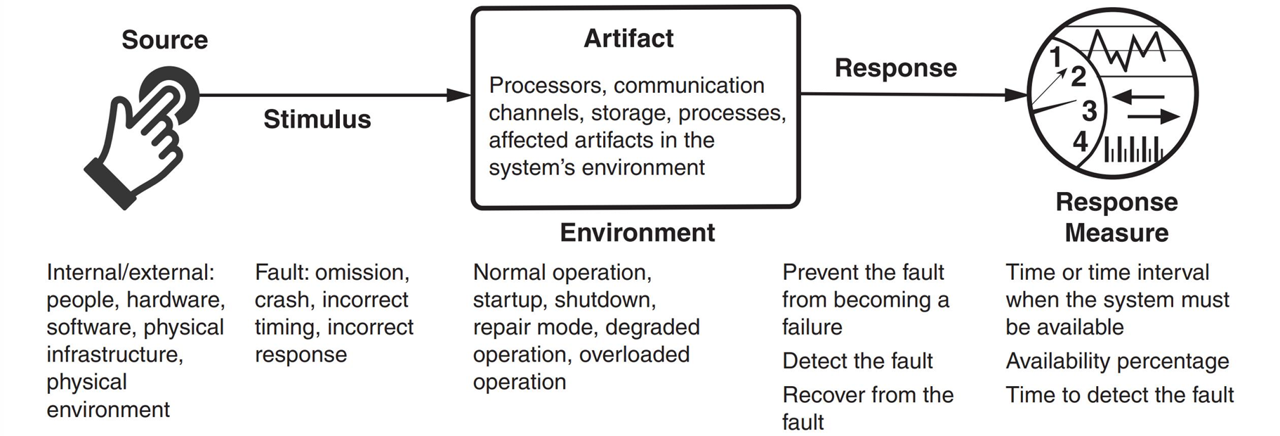
\includegraphics[width=1\linewidth]{QAScenarios}}

\textbf{Example Non-Functional Requirements and Metrics}
\begin{itemize}
    \item \textbf{Availability}: System readiness to perform tasks, reliability and recoverability. \textit{Metrics}: Availability \%, time to detect/repair faults, etc. (QA Scenario: E.g. 1. Source: server, 2. Stimulus: crashes, 3. Artifact: the server software, 4. Environment: any operational state, 5. Response: detects the abnormal state and re-routes traffic to another server, 6. Response measure: within 5 seconds of the server becoming unresponsive).
    \item \textbf{Performance}: System responsiveness. \textit{Metrics}: Latency, throughput etc.
    \item \textbf{Modifiability}: Cost and effort. \textit{Metrics}: Elapsed time, new defects introduced.
    \item \textbf{Deployability}: The ease of deploying and rolling back system changes. \textit{Metrics}: Cost, percentage of failed deployments, cycle time, etc.
    \item \textbf{Security}: Protecting data and systems from unauthorized access. (CIA Triad) \textit{Metrics}: Accuracy of attack detection, size of trusted execution 
\end{itemize}

\subsubsection{Requirement Engineering Process Models}
\textbf{Agile Approaches}: Agile avoids detailed requirements documents due to rapid changes. Relies on user stories and frequent stakeholder feedback. Iterative feedback, collaboration. Short supporting documents may still define business and dependability requirements. \\
\textbf{Plan-Driven Approaches}: Follow a structured process model. RE phase is completed before implementation. Produces a requirements document, often part of the development contract. Focus on detailed specification and validation  \\ \smallskip
\textbf{SRS: Software Requirements Specification}: Central document of what to implement. Detailed specification of system/user requirements. Output of RE. \\ \smallskip
\textbf{Stakeholders}: impacted / influencing requirements. Start with "baseline" stakeholders (e.g., users, decision-makers). Explore network to identify more.


\subsubsection{RE Key Activities - 3Cs of User Stories}
\centerline{Elicitation and analysis $\rightarrow$ Conversation (w. client).} 
\centerline{Specification $\rightarrow$ Card (description).}
\centerline{Validation $\rightarrow$ Confirmation (acceptance tests to determine completeness).} \smallskip

 \begin{enumerate}[leftmargin=2mm,labelindent=1mm,labelsep=1mm, itemsep = 0.5pt, before=\justifying]
    \item \textbf{Elicitation and Analysis}: \underline{Get Requirements working w. stakeholders}. \\
    \textit{Elicitation techniques}: Interview, Existing Docs Analysis, (user-story) workshops -- multiple stakeholders \& resource intensive, FGs (users), prototype, observe -- discover implicit req. reflecting actual ways. Personas.
    \begin{itemize}
\item \textbf{RE Elicitation and Analysis Model}: \\
     \textit{Requirements Discovery} (Interact w. stakeholders to uncover needs) $\rightarrow$ 
    \textit{Classification and Organization} (Group req. to coherent clusters) $\rightarrow$
    \textit{Prioritization and Negotiation} (Resolve conflicts, prioritize req) $\rightarrow$
    \textit{Documentation} (Record requirements for next iteration) $\rightarrow$ (repeat)
\end{itemize}
    \item \textbf{Specification}: \underline{Convert Requirements to standard form (user-centric view).} \\
     \textit{User Stories}: represent customer requirements ($<$As `user-type', want `goal', to `reason'.$>$) \textbf{Three Cs} - card, convo, confirm. \textbf{Epics} -- too large user stories to be split later. Include notes, NFRs (constraints). \\
    \textit{Use Cases}: interaction btwn actor \& system (e.g. check in flight). UML $\rightarrow$ use case diagram. May encompass multiple scenarios (single instance of usage e.g normal flow, crash, others etc). Natural Language -- use standard format, consistency, associate rationales, avoid jargon.
    \begin{itemize}
\item \textbf{User vs. System Requirements}: \textbf{UR}: High-level, no software jargon descriptions of external behaviour of system. \textbf{SR}: Complete, detailed description of whole system, external behavior and operational constraints.
\end{itemize}
    \item \textbf{Validation}: \underline{Ensure requirements actually define desired system}. \\
     (\textit{Agile}: freq comm. w stakeholder, \textit{Plan}: check unclarities in req. document). \textbf{Techniques}: \textit{Informal Reviews}: Peer review, colleague reviews requirements. Informal feedback collection (e.g., deskchecks, walkthroughs). \textit{Formal Reviews}: Systematic analysis by a team of reviewers, roles: Moderator, reader, inspectors. Techniques: Defect checklists, requirement-by-requirement reviews. \\
      \textbf{Requirement document checks}: \textit{Validity}: reflect real user current needs. \textit{Consistency}: Avoid contradictory req. \textit{Completeness}.  \textit{Realism}: feasible, within budget, tech constraints. \textit{Verifiability}: testable. \\
	    \textbf{Feasibility Study}: short study to assess: alignment with organizational objectives, budget and schedule, Integration with existing systems. \\
	    \textbf{Prototyping}: Quick version of system to validate requirements and design decisions. Reduce post-delivery changes by allowing early experimentation.
	    \begin{itemize}
\item \textbf{Requirements Change Management (During Validation)}: \\
    \textit{Established Plan for to manage evolving requirements.} \\
    Unique identification of requirements (to cross-reference). \\
    Established change management process to assess impact and cost. \\
    Traceability policies to link requirements to design. \\
    Tool support for managing requirements
\end{itemize}
\end{enumerate}	    

\subsubsection{Specification and Validation}

\begin{itemize}    
	    \item \textbf{Use Cases vs User Stories} (Use Cases -- Plan-Driven): Specify functional requirements and serve as test bases. (User Stories -- Agile): Act as placeholders for implementation, elaborated into acceptance tests.
	    \item \textbf{Requirements as a Basis for Testing}: Requirements should be testable and used to derive test cases. User stories, cases as foundations for acceptance tests.
	    \item \textbf{V-Model (Plan-Driven Approaches)}: In plan-driven approaches, \underline{requirements validation} also has test planning, and aligns with \underline{testing phases} in the V-Model. (I.e. User Requirement + acceptance test planning $\leftrightarrow$ acceptance test, Functional Req $\leftrightarrow$ System Test, Architecture $\leftrightarrow$ integration test, Design $\leftrightarrow$ Unit Test.) Horizontal axis is time. Represented as V - shape to match.
    \item \textbf{Spiral Model}: iterative, plan-driven RE process model. Expands requirements incrementally, focusing on high-level business needs early and detailed system requirements later. Outputs SRS. Can incorporate agile in later iterations. (From inside spiral outwards. Repeated cycle of Elicitation, Specification and Validation) 
	\end{itemize}


\subsection{4. \underline{System Modeling and Software Architecture}}

\subsubsection{Systems Modeling}
Develop abstract models of a system. Means to an end (developing software). 
\begin{itemize}
	\item Emphasized in plan-driven, in agile used in lightweight manner (“just enough”).
	\item Formal models (mathematical) can be developed for auto verification.
       \item Models created during requirements engineering, system design, and post-implementation documentation.
       \item \textbf{Abstraction vs Representation}: Abstraction simplifies systems, omits details. Representation maintains all system information.
       \item \textbf{Different perspectives}: External, Interaction, Structural, Behavioral.
\end{itemize}

\subsubsection{Modeling Languages {\scriptsize (UML, C4, others: BPMN, SysML, etc.)}}
\textbf{UML (Unified Modeling Language) Key Diagrams}:
\begin{itemize}
  	\setlength\itemsep{-0.1em}
	\item Class Diagrams: Show object classes and associations.
	\item Sequence Diagrams: Show interactions btw. actors \& components.
	\item Activity Diagrams: Show process or data flow activities.
	\item State Diagrams: Show system reactions to events.
	\item Use Case Diagrams: Show interactions btwn system \& environm.
\end{itemize}

\smallskip
\textbf{C4 Model}: Agile Architectural Modeling. For software architectures. Do "just enough" design / upfront thinking for starting point/ general direction.
\begin{itemize}
	\item Hierarchical architectural modeling (4Cs): System Context, Containers, Components, Code. Notation Independent.
\end{itemize}
    
\begin{itemize}
        \item \textit{System Context diagram} $\rightarrow$ starting point, how software fits into world.
        \item  \textit{Container diagram} $\rightarrow$ software system, high level building blocks.
        \item  \textit{Component diagram} $\rightarrow$ individual container, decomposes containers to identify major structural building blocks (components). Not recommend unless adds value.
       \item  \textit{Code diagram} (e.g. UML class) $\rightarrow$ indivdual component implementation. Not recommended for C4 / Agile context use.
\end{itemize}

\centerline{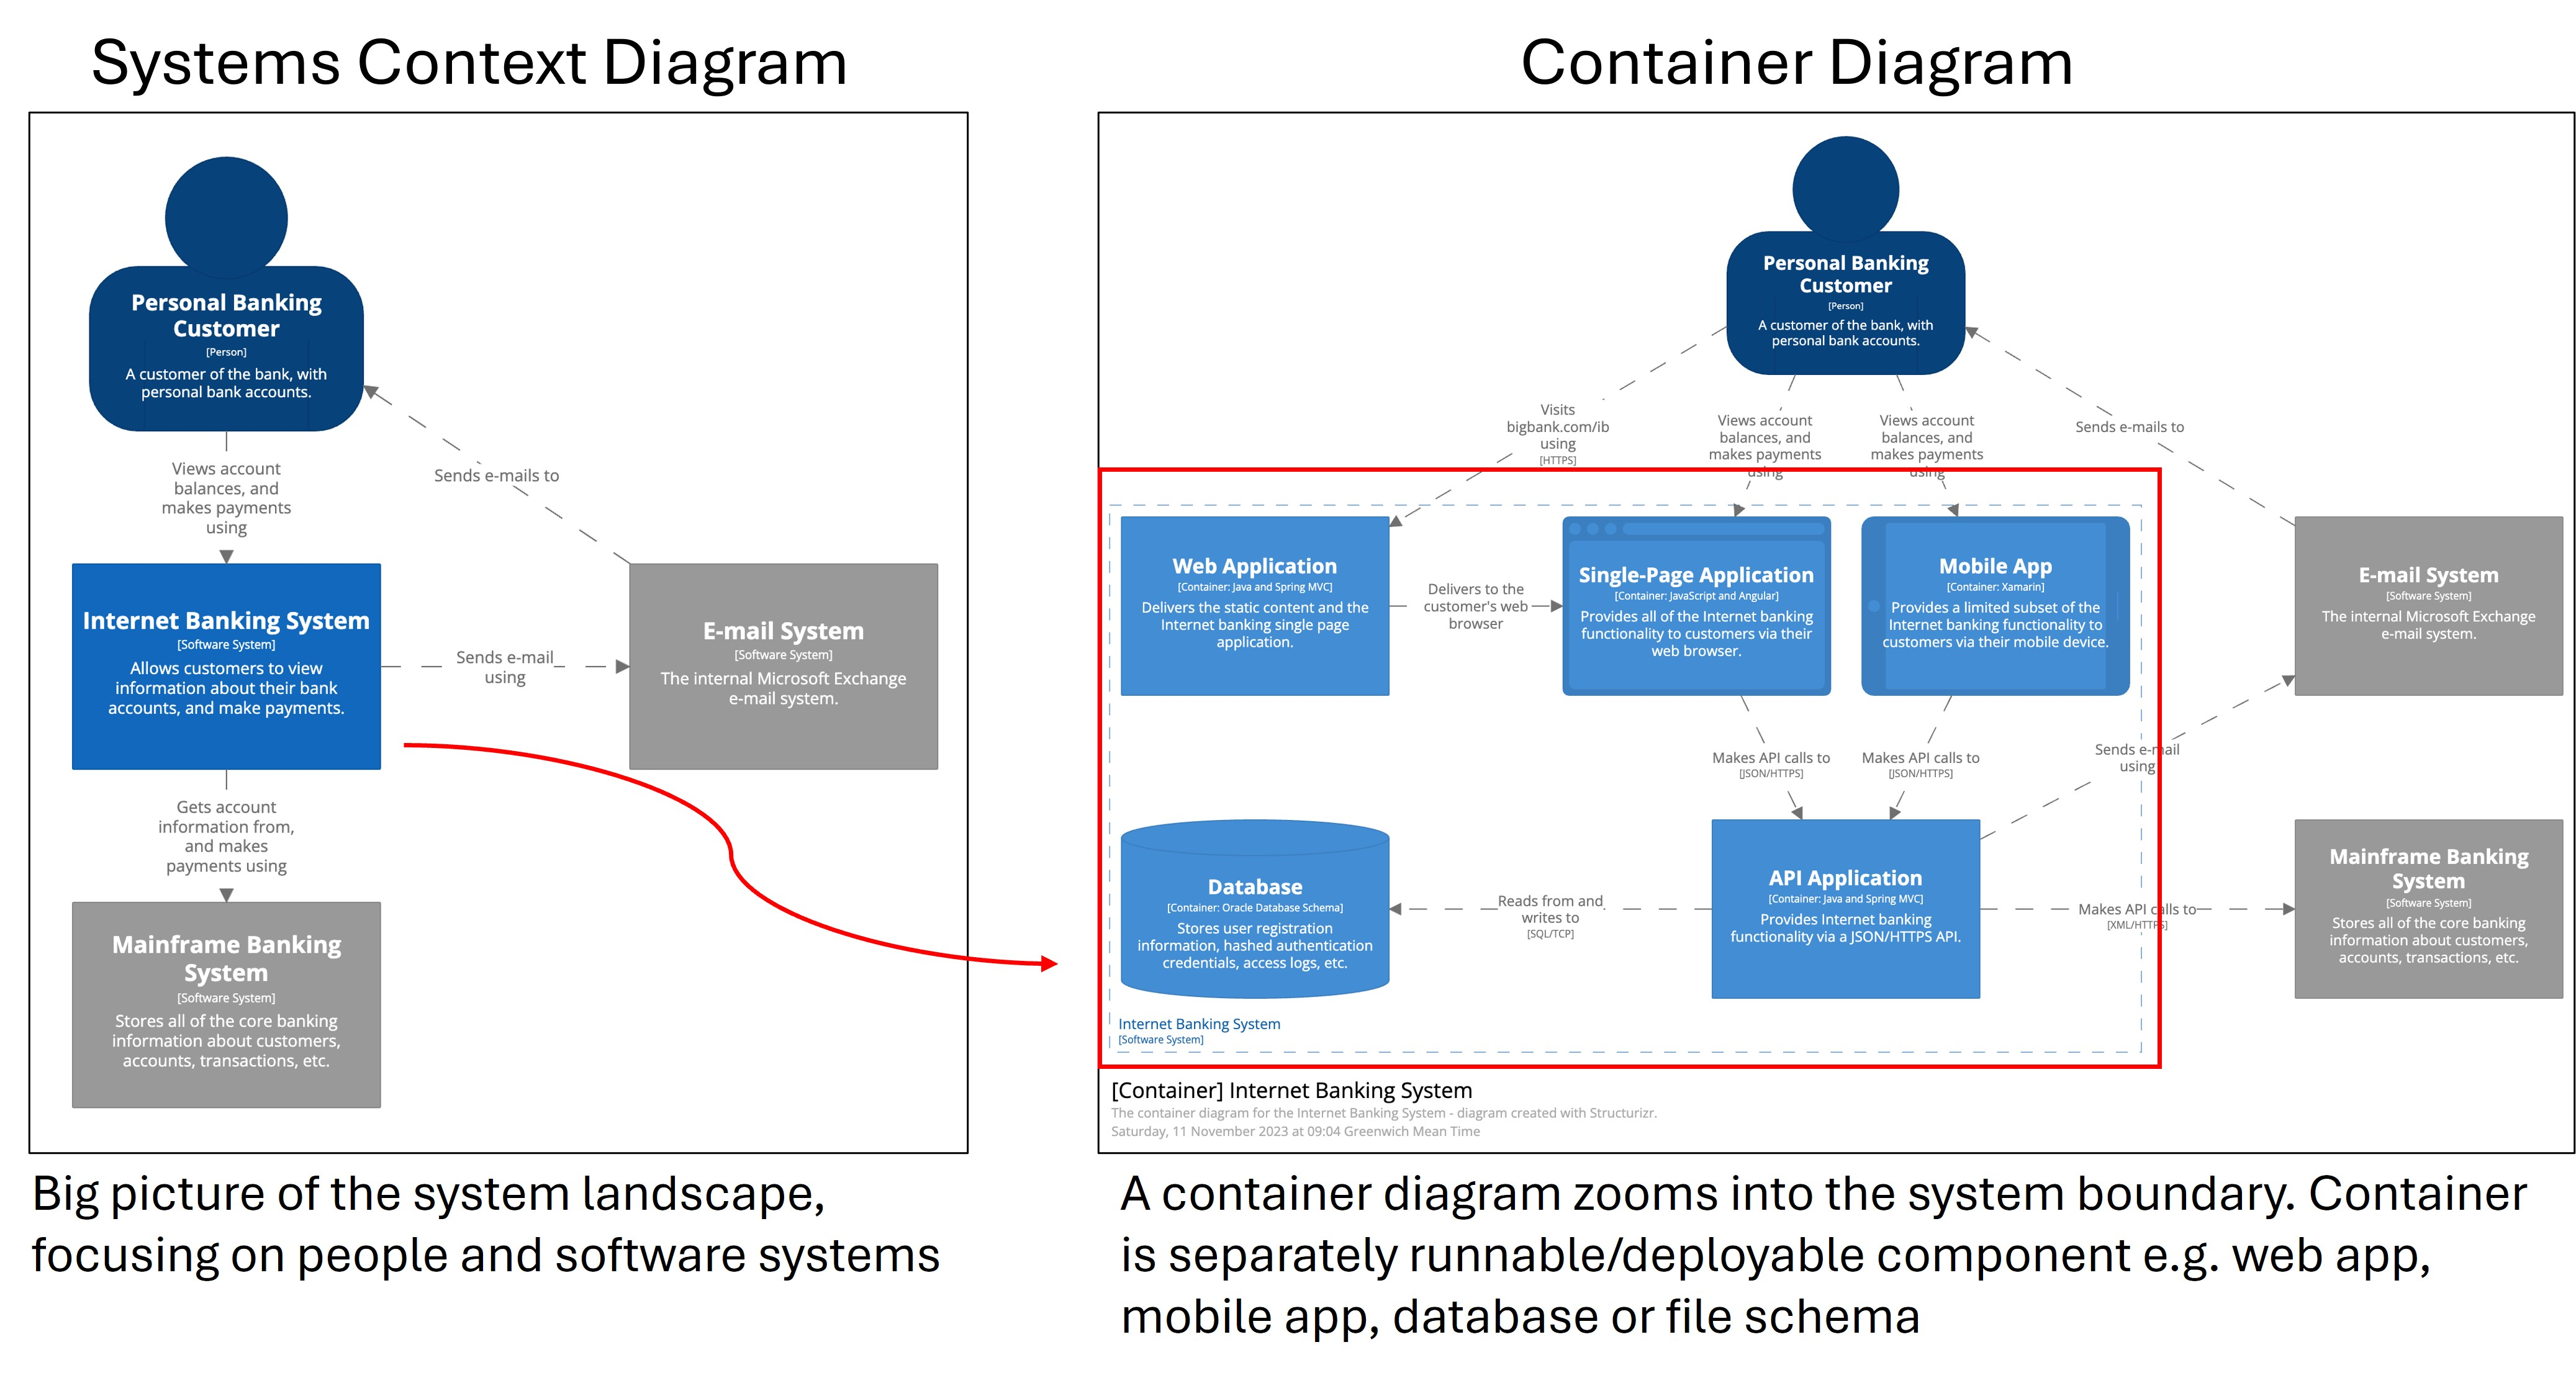
\includegraphics[width=0.5\linewidth]{c4}}


\subsubsection{Software Architecture  {\scriptsize (overall structure of a system, part of software design)}}
\begin{itemize}
	\item \textbf{Influences quality attributes, modifiability, and communication} among stakeholders. Mitigate highest priority risks. Difficult to change later.
      \item \textbf{Architectural Drivers: Architecturally Significant Requirements (ASRs)}: Requirements that significantly impact architecture. Non-functional req. (e.g. availability, performance) often ASRs. Functionality must have major influence on architecture. (E.g. system should provide five nines (99.999 percent) availability). 
\end{itemize}
Often, system architecture modeled informally w. simple block diagrams.

\subsubsection{Architectural Reasons and Consequences}
\begin{itemize}
    \item \textbf{Quality Attributes}: Architecture significantly influences whether system meets quality attributes (non-functional requirements). (E.g. \textit{High Performance} -- require managing time-based behavior and shared resource access, \textit{Safety and Security}... )
    \item \textbf{Modifiability and Change}: Modifiability is a critical quality attribute. Requires assigning responsibilities to components to limit the impact of changes.
    \textit{Categories of changes}: Local -- affect only single component, Non-local -- Affect multiple components (e.g. UI). Architectural Change -- Affects entire system (e.g., single-thread to multi-thread). Good architecture ensures most changes local or non-local.
    \item \textbf{Communication Among Stakeholders}: Architecture as common abstraction for mutual understanding, negotiation, and consensus.
    \item \textbf{Additional}: Enables reasoning of cost, schedule, basis for reusable models in product lines, focuses on component assembly, channels developer creativity by restricting design alternatives, foundation for training new team members, enable early prediction of system qualities, defines constraints for subsequent implementation, influences org structure (Conway’s Law), supports incremental dev.
    \item \textbf{Conway’s Law}: Organizations design systems that mirror their communication structures -- Architecture often forms basis for work-breakdown structures.
\end{itemize}

\subsubsection{Attribute Driven Design (ADD): Architecture Patterns and Tatics}
Architecture is a tradeoff of attributes. \\
\textbf{Architectural tactic}: design decision that influences a quality attribute. \\
\textbf{Architectural Patterns}: Established architectural solution, may comprise multiple architectural tactics. Often found useful over time, documented and disseminated.
\begin{itemize}
\item \textbf{Attribute-Driven Design (ADD)}: Systematic approach to architecture design. Each design iteration, address an ASR. \\
\textbf{Steps}: Identify ASRs $\rightarrow$ set iteration goals (satisfy which set of ASRs) $\rightarrow$ choose target structure $\rightarrow$ select designs (choose tatics, patterns, most difficult) $\rightarrow$ instantiate patterns in context $\rightarrow$ record decisions $\rightarrow$ validate, repeat.
\end{itemize}
\begin{itemize}
\item \textbf{Antipattern -- Big Ball of Mud}: Common in practice. Lack of architectural design, Business pressure, Erosion of architecture over time. 
Poor maintainability, extensibility (Quality Attributes)
\end{itemize}

\subsubsection{Common Architectural Patterns}
\begin{itemize}
	\item \textbf{Layered Architecture}: Structures systems into layers with defined interfaces. Layer only uses layer directly beneath, through public interface. (constraints may be violated e.g. for performance, layer bridging, upper layer bypass lower layers). \\
	 \textit{Pros}: portability (to diff env/OS), modifiability (lower layers changeable under hood, less interfaces to understand), reuse\\
	 \textit{Cons}: Layering possible performance penalty. If not properly designed, can impede (missing nec. low level abstraction needed at higher level).
	 
      \item \textbf{Pipe-and-Filter}: Processes data through independent filters connected by pipes. \textit{Filters}: processing components, take input, produce output, no assumption on other filters, stateless. \textit{Pipes}: connect multiple filters with each other. (E.g. MailMan - add header, digest, archive, outgoing). \\
      \textit{Pros}: modifiability (independent filters) and reconfigurability, evolution (add/combine filers differently) \\
      \textit{Cons}: format data transfer must be set. performance as every filter must parse input convert to output format.
      
      \item \textbf{Model-Centered}: Independent components interact with a central model than each other. Repository style. (E.g. IDEs). \\
      \textit{Pros}: components can be independent. highly modifiable. concurrency. State/data manged consistently (in one place).  \\
      \textit{Cons}: model/repo is single point of failure. change to model $=$ many changes. Distributing repo can be difficult. \\  \\
      \textbf{MVC design pattern}: ''instantiation" of model-centered, goal of MVC to separate model (business logic) from UI (controller/view).
      
      \item \textbf{Microkernel (Plug-in)}: Base system, plug-in components (e.g. web browser). \\
      \textit{Pros}: modifiability, extensibility, testability. Plugins can be developed, tested, evolved by diff. teams independently. \\
      \textit{Cons}: can introduce security /privacy vulnerabilities \\
      
      \item \textbf{Client-Server}: central server, provide service to multiple distributed clients. Client request service, server cannot initiate. (E.g. web server) \textit{Discovery}: client use discovery service, server respond w. agreed protocol. \textit{Interaction}: client sends request, server process, respond.   \\
      \textit{Pros}: Low coupling btwn server clients, no coupling among clients. Easily scale no. clients and server. Both can evolve indptly.

      \item \textbf{Microservices}: Independently deployable services communicating via APIs. Typically stateless, small teams, small code bases. Service dependencies acyclic. Popularized by large companies. Goal - decoupling, microservices expected to be independent w own domain/workflow. typically smaller than services in SOA. \\
      \textit{Pros}: quick time to market, indiv. deployability, test, scalability. \\
      \textit{Cons}: network comm. overhead, complex transactions, challenge in design /maintain sea of microservices\\
\end{itemize}

\centerline{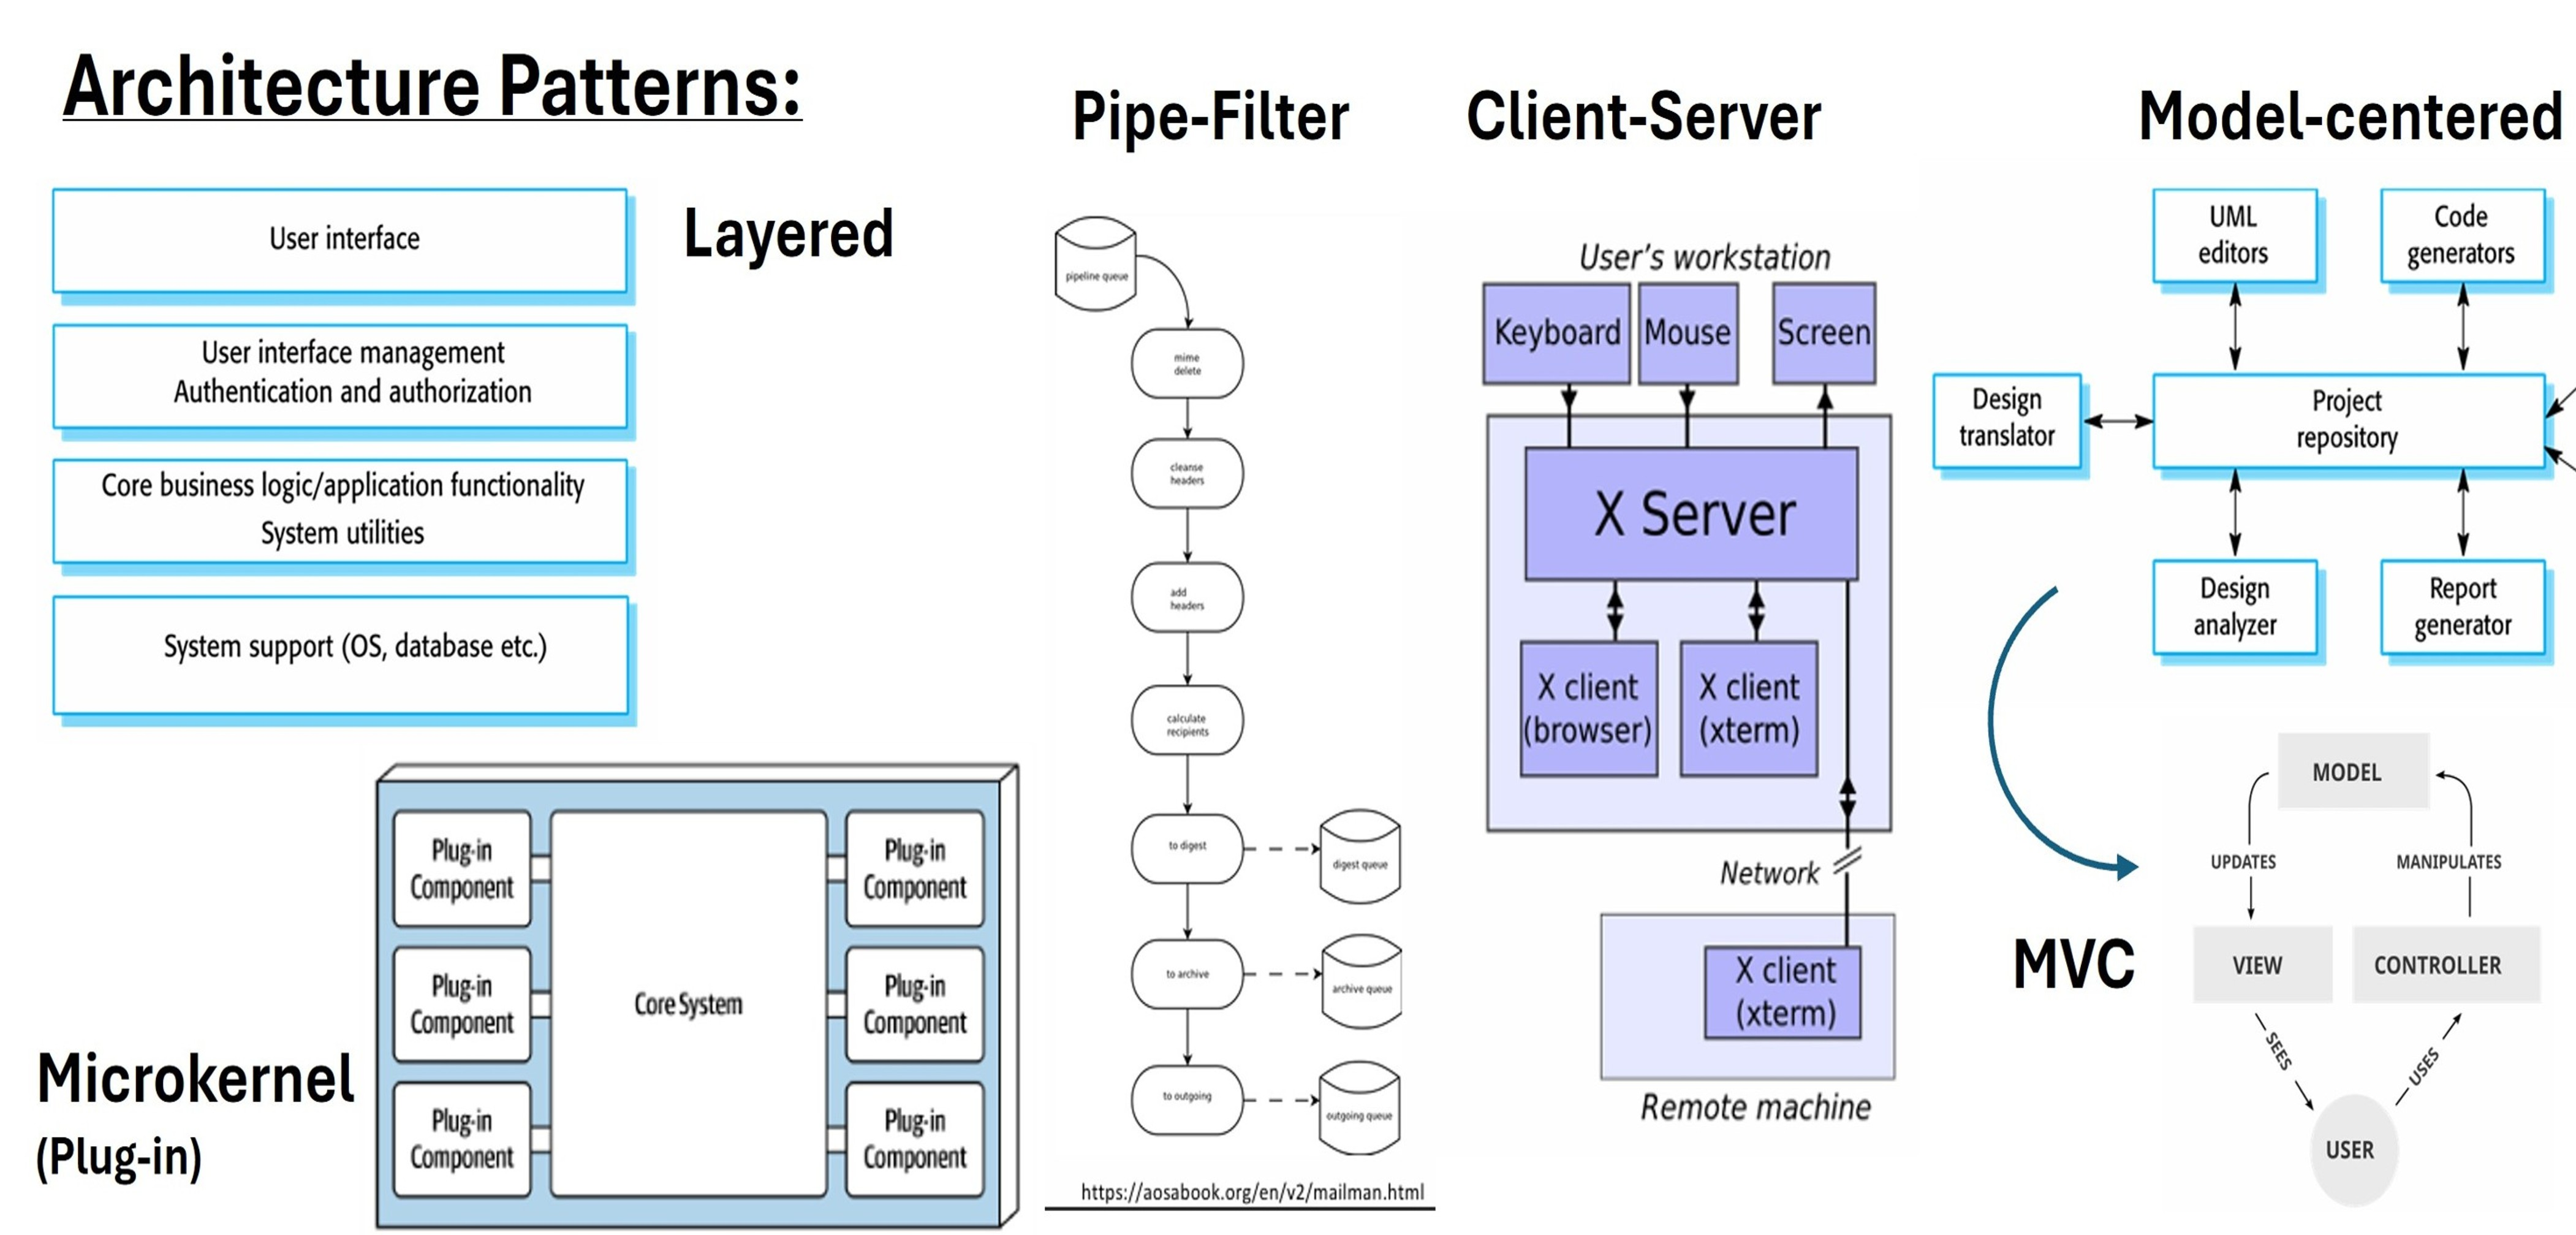
\includegraphics[width=1\linewidth]{architecture2}}
\smallskip
\textbf{Monoliths vs. Service-Oriented Architecture (SOA)}: Monolith typically single deployable unit (diff. way of partition e.g. layered archi.). SOA for distributed-architecture styles, services separately deployed, only interact over interfaces, network. Related to microservices.

\subsubsection{Architectural Tactics}
Tatics are design decisions that influence quality attributes. E.g.
\begin{itemize}
  	\setlength\itemsep{-0.2em}
	\item \textit{Availability Tactics}: Detect faults (monitoring, heartbeat), recover (redundant spare, rollback), prevent faults (ACID transactions, remove from service).
	\item \textit{Performance Tactics}: Control Resource Demand: (Manage work requests, limit event response, bound execution times), Manage Resources: (maintain multiple copies of data, schedule resources, bound queue sizes, introduce concurrency).
\end{itemize}

% \centerline{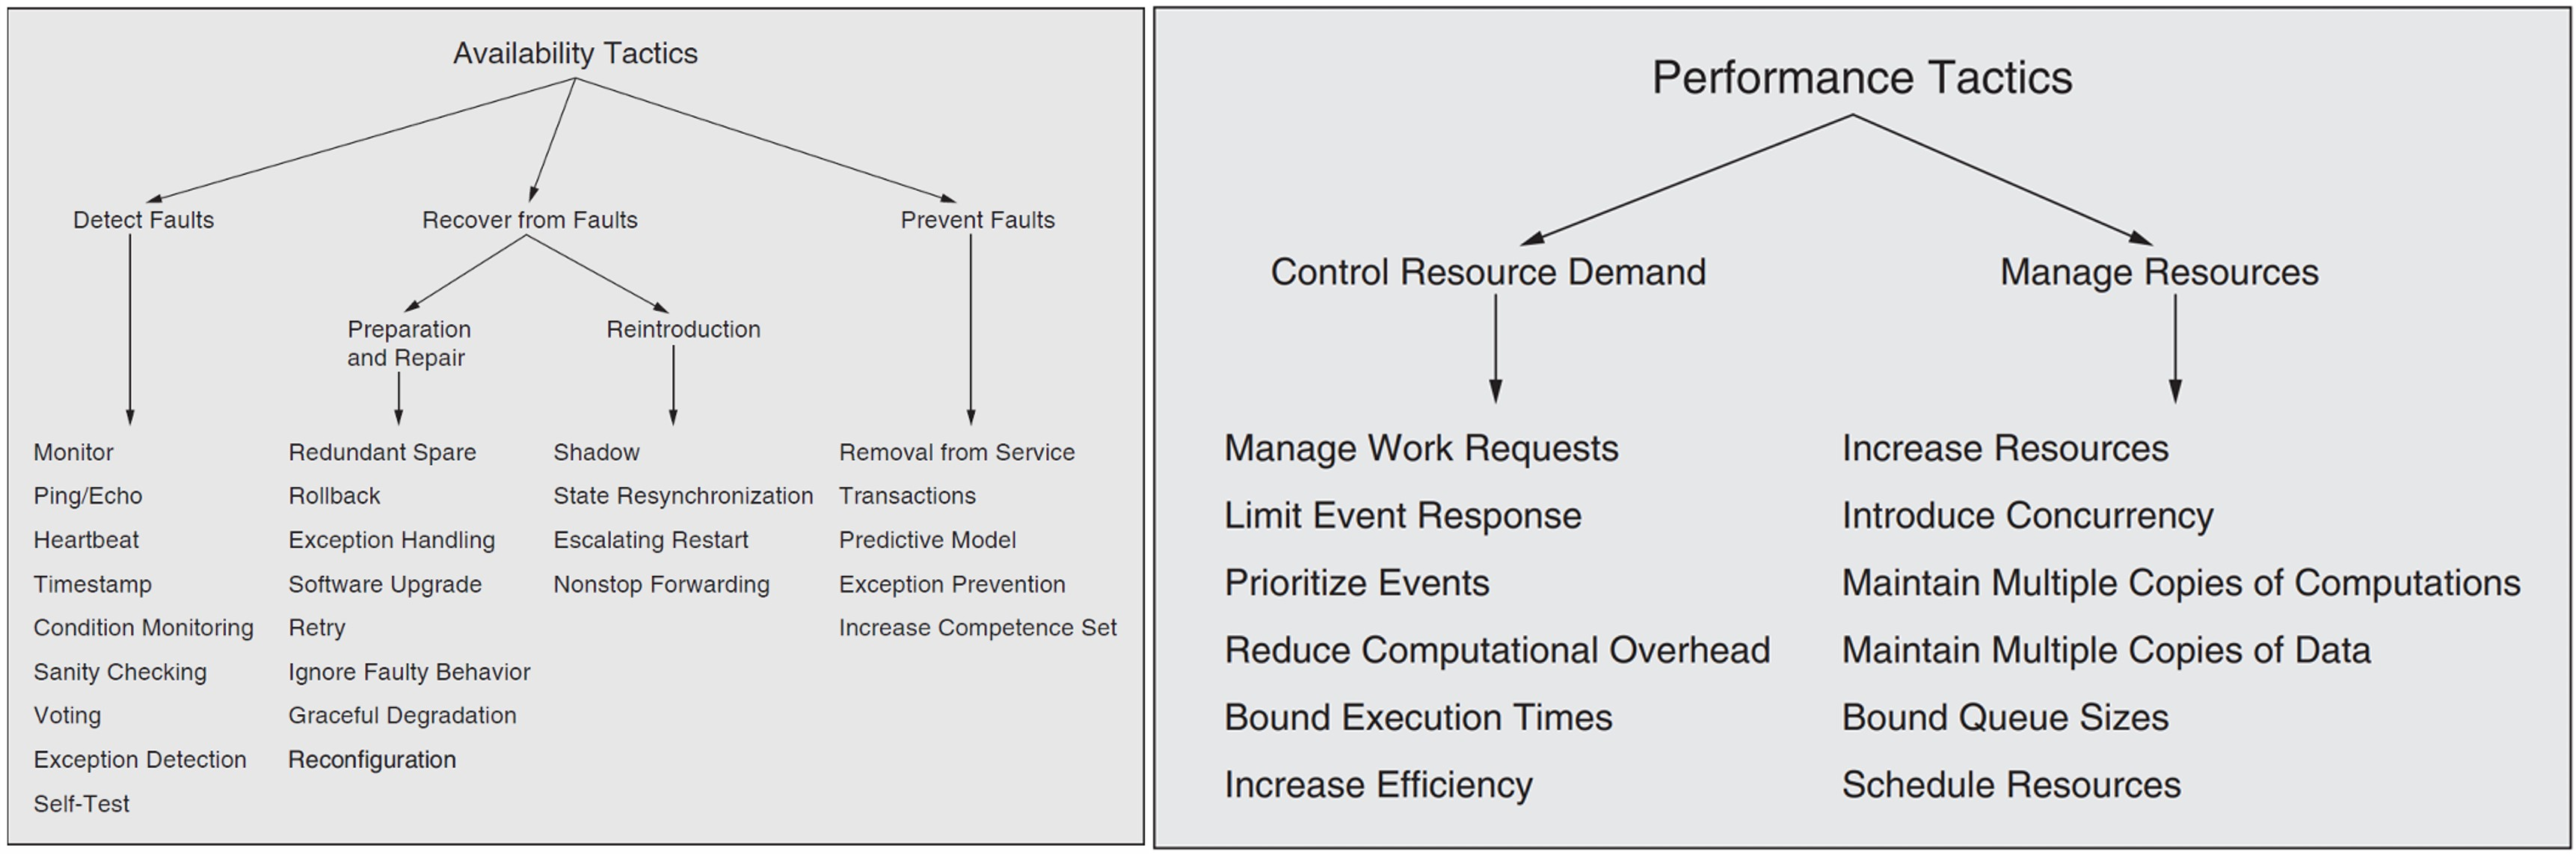
\includegraphics[width=1\linewidth]{tatics}}

\textbf{"20 minutes rule"}: Continuous learning essential for staying updated.


\columnbreak

% TO DO FROM HEREEEEEEEEEEEE

\subsection{5. \underline{Software Testing}}
\textbf{Purpose of Testing}: \textit{Defect Testing}: Find bugs in software. (Tests show presence, but never absence.) \textit{Validation Testing}: Ensure system meets user requirements.

\begin{itemize}
	\item \textbf{Verification vs. Validation}: 
		\textit{Verify}: Build product right, conforms to specification. 
	       \textit{Validate}: Build right product, software meets user needs.
	\item \textbf{Test Case}: A test case consists of: 
		\textit{Test Input}: Arguments, system state, or actions, \textit{Test Oracle}: Mechanism, determine test pass or fail.
    \item \textbf{Test Oracle}: Can check functional properties (e.g., correctness) or non-functional properties (e.g., performance, security).
    \item \textbf{Manual vs. Automated Testing}: \textit{Automated}: Use tools to auto generate inputs and apply oracles (e.g., JUnit). \textit{Manual}: Tester manually inputs test cases and acts as oracle. (`Traditional' -  auto as in test automation).
    \item \textbf{Pesticide Paradox (Diminishing Return)}: `Every method used to prevent/find bugs leaves residue of subtler bugs which those methods ineffectual'. Diff testing methods have pros, cons. Use many, similar to pests build immunity.
    \end{itemize}

\subsubsection{Testing Levels, Flaky Tests}
\begin{enumerate}[leftmargin=2mm,labelindent=1mm,labelsep=1mm, itemsep = 0.5pt, before=\justifying]
    \item \textbf{Unit Tests}: Test indiv. components (e.g., single method/class). \\
    	\textit{Pros}: Fast execution, easy control, write (no additional setup (e.g., no DB). \\
    	\textit{Cons}: Lack realism, don’t represent real system execution. May miss integration bugs, often require mocks to simulate external dependencies.

    \item \textbf{Integration Tests}: Test interactions btw. multiple components. Focus on integrating target cmpnt. w. external cmpnt. (e.g., ext DB, web service). - (e.g. SQLancer test query plan converted to expected internal representation.)

    \item \textbf{System Tests}: Test entire system as whole. \textit{Pro}: realistic test env. \textit{Cons}: slower execution, harder to write  (complex setup), prone to flakiness (non-deterministic results). (e.g: Ensuring SQLancer compatibility with database system.)
\end{enumerate}
\begin{itemize}
    \item \textbf{Test Flakiness}: Pass/fail non-deterministically. Low result confidence. \\
    \textit{Causes}: Concurrency issue (e.g., race conditions), async waits (e.g., not properly waiting for server responses), test order dependencies (e.g., improper cleanup), test timeouts, resource leaks. (e.g, test fail from \texttt{ConcurrentModificationException} in multi-threaded code.)

    \item \textbf{Test Pyramid}: strategy for balancing test granularity. Many small, fast unit tests as base. Fewer integration, system tests.
	 \textit{Antipatterns}: Too many high-level tests, slow execution, maintenance challenges.
\end{itemize}
% \centerline{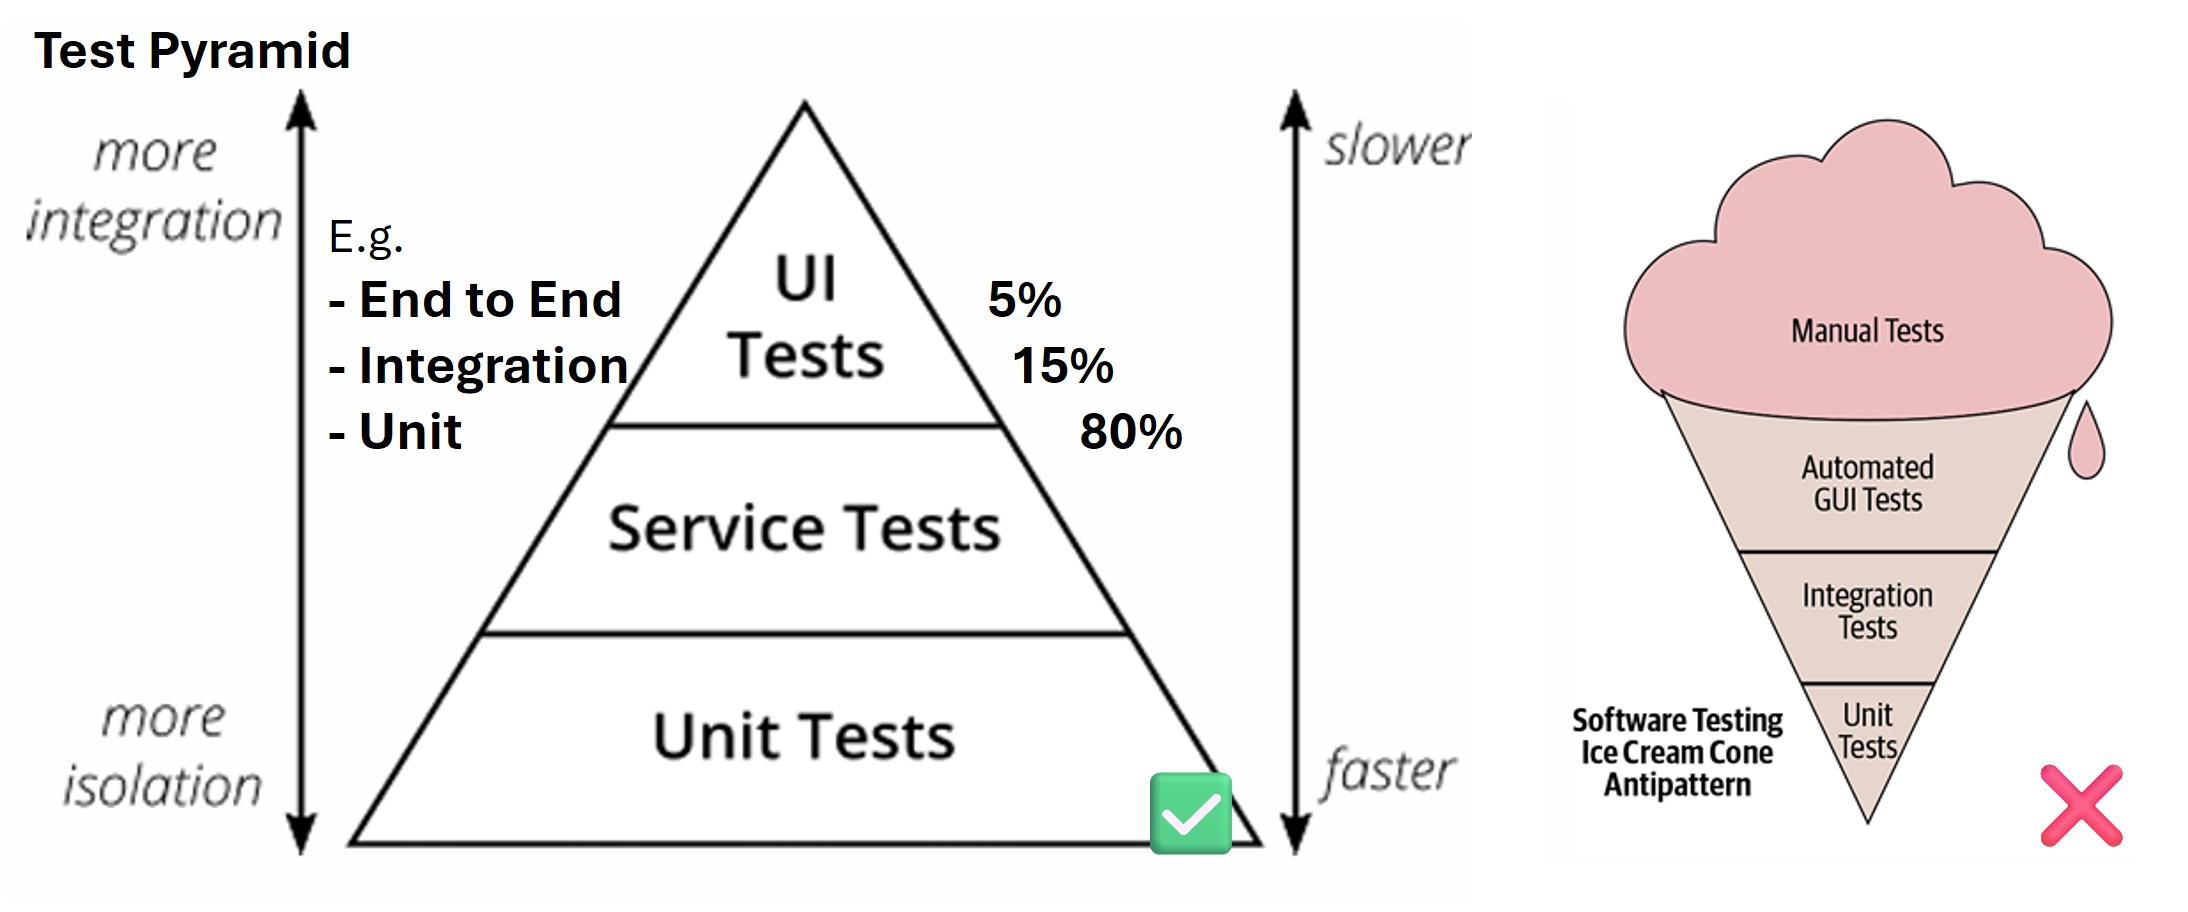
\includegraphics[width=0.9\linewidth]{testPyramid}}
\begin{itemize}
    \item \textbf{E.g. Test Sizes at Google}: Tests classified by size to for efficiency, determinism. \\
     \textit{Small}: Single process/thread, no I/O, fast, deterministic. \\
      \textit{Medium}: Multiple processes, allow localhost network calls. \\
      \textit{Large}: No restrictions, slower, less deterministic.
\end{itemize}

\subsubsection{Testing and Processes}
\begin{itemize}
	\item \textbf{Plan Driven Development}:
\begin{itemize}
\item \textbf{V-Model}: extension of waterfall model. Tests planned alongside RE. 
    \item \textbf{User Acceptance Testing}: validate system meets user req, w customer participation. In \textit{plan driven}, explicit phase after system implementation. In \textit{agile}, UAT is interleaved (e.g., acceptance criteria in user stories).
\end{itemize}

    \item \textbf{Test-Driven Development (TDD)}: Emphasized by XP. Use as design process, focus `happy path'. 
    	\textit{Pros}: Focus on req, provide quick feedback. Encourages testable code, allows incremental exploration. 
    	\\ \textit{Steps:} Write test $\rightarrow$ ensure fails $\rightarrow$ simplest code to pass $\rightarrow$ refactor.
	\\ \textit{When to Use}: Useful for complex prob, unclear soln (incremental experimentation). Less useful if solution already clear. \\
	Schools of thought: (Classicist/Detroit, Inside-out start e.g. business rules $\rightarrow$ UI). (London/Mockist Outside-In: Start outside, use mocks).

    \item \textbf{Black-box vs. White-box Testing}: \\
    	\textit{Black-box `specification testing'}: No internal info, based on requirements. \\
    	\textit{White-box `structural testing'}: Internal info, focus code structure, logic.
\end{itemize}

\subsubsection{Black-box Testing (Specification Based Testing)}
\begin{itemize}
    \item \textbf{Specification-based Testing}: Derive from requirements (e.g., user stories, use cases, docs). Functional \& non-functional requirements. \\
	 \textit{Testing Workflow}: Understand requirements (input, output), explore program (functionality), identify partitions (eqv classes of input/output), analyze boundaries, devise and automate test cases, augment test suite with common bugs.
    \item \textbf{Equivalence Partitioning}: Divides inputs into equivalent classes. Output partition may help spot input partition. Combinations of partitions of individual inputs.
    \begin{itemize}
		\item E.g. Partitions for STR: null, empty, single-char string, multi-char string.
	\end{itemize}
    \item \textbf{Boundary Value Analysis}: Inputs at boundaries more likely to trigger bugs (e.g. off by one errors). Program behavior changes when going from one boundary to the other. Tests edge cases (e.g., min/max).
    \begin{itemize}
		\item E.g. For given partitions, choose boundaries. ($+1, -1, =$)
	\end{itemize}
\end{itemize}

\subsubsection{White-box Testing (Structural + Mutation Testing)}

\begin{itemize}
    \item \textbf{Structural Testing}: use source code to guide testing. Catch requirement independent implementation aspect (e.g. cache, DSA). Focus on coverage criteria.
    \item \textbf{Coverage Criteria}:
    
    \begin{itemize}
		\item \textit{Line Coverage} (percentage executed).
		\item \textit{Branch Coverage} (branch percentage executed).
		\item \textit{Branch $+$ Condition Coverage}:  Considers every condition of each branch statement. E.g. \texttt{if ($a || b$)}. Condition coverage does not imply branch coverage. 
		\item \textit{Path Coverage}: Strongest criterion. Often impossible (e.g. loop). In simple function with 10 conditions, number of paths $= 1024$
		\item \textit{Modified Condition/Decision Coverage (MC/DC) Coverage}: Test important combinations of conditions, with less cost.
		\item Overall, Path Coverage $>$ MC/DC $>$ Branch$+$Condition ... (subsumes/includes)
	\end{itemize}    
\end{itemize} 
\subsubsection{MC/DC Coverage}
\[ \frac{\text{Number of conditions independently tested to affect decision outcome}}{\text{total number of conditions in decisions}} \times 100\%\] 
\begin{itemize}
\item For each decision (Boolean expression), identify all conditions. Count conditions:
	\begin{enumerate}[itemsep = 0pt, topsep=0pt]
	\item Tested with both true and false values.
	\item Proven to independently affect the decision's result.
	\end{enumerate}
\item (For a decision with $n$ conditions, $n+1$ test cases lower bound to demonstrate independence for each condition.)
\end{itemize}



\centerline{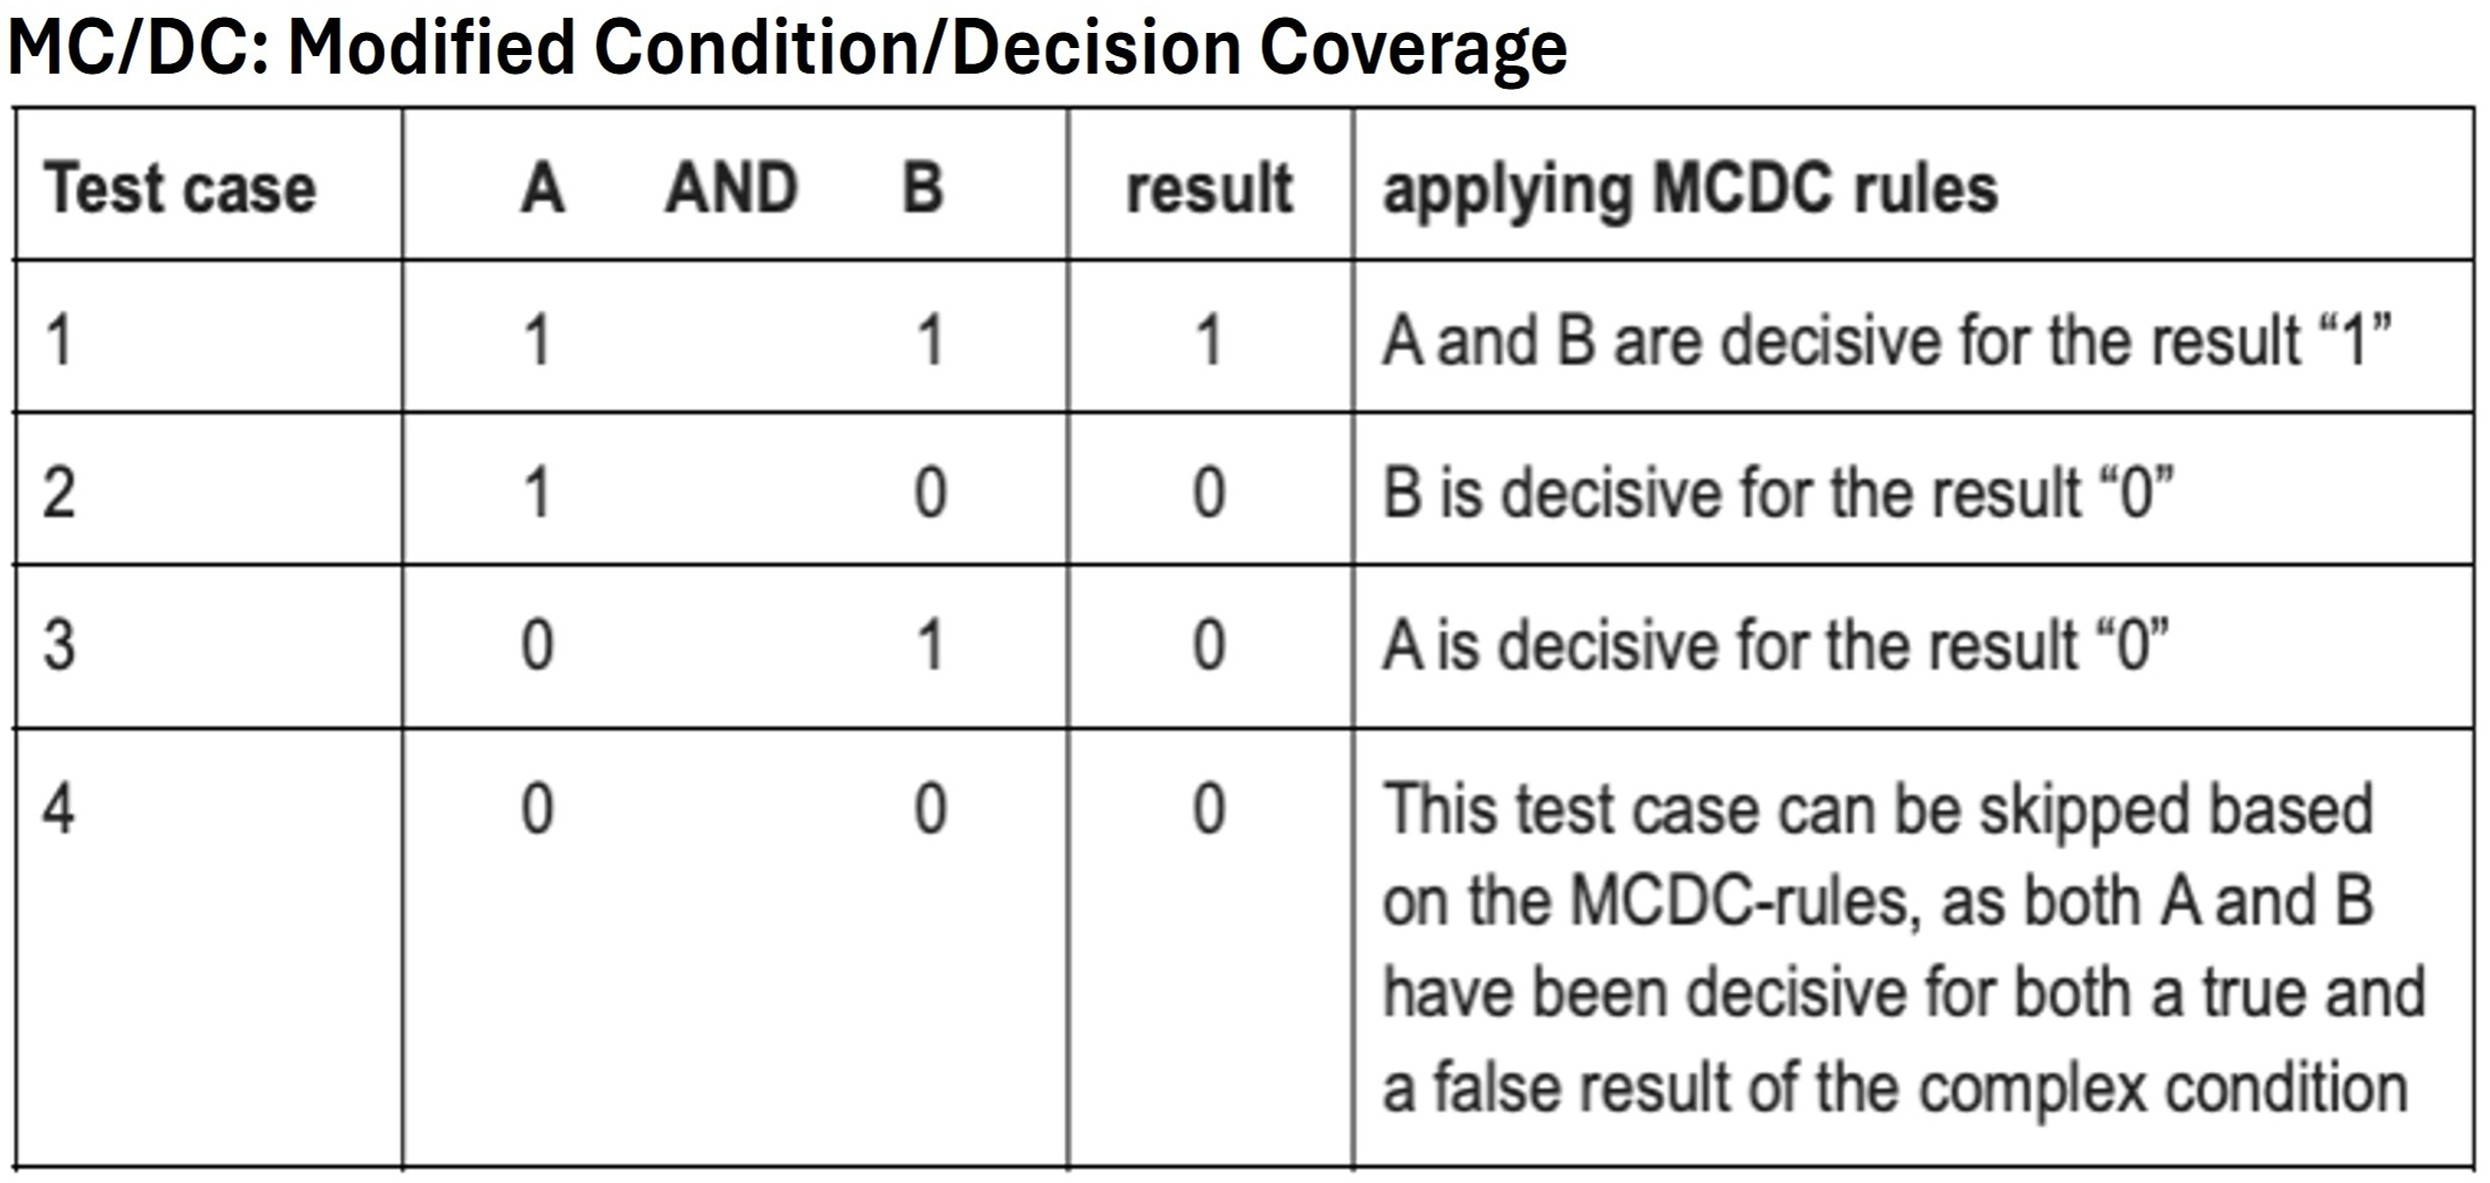
\includegraphics[width=1\linewidth]{MCDC2}}

\begin{itemize}
\item \textbf{Mutation Testing}: checks how good test cases are by intentionally adding small bugs (mutants) to code and seeing if tests can catch/kill them. \\
\textbf{Steps}: Select statement in code, mutate code, run test suite, record outcome. Undo change, repeat. Calculate mutation score: \(\frac{\text{\#killed mutants}}{\text{\#mutants}} \times 100\). \\
	\textit{Pros}: Identify undertested code.\\
	\textit{Cons}: Comptn expensive; equivalent mutants may not change behavior.
\end{itemize}

% -------------------------------------------------------------------------------------------------------------%

% TO DO FROM HEREEEEEEEEEEEE


\subsection{6. \underline{Debugging and Fault Localization}}

\subsubsection{Debugging}
\begin{itemize}[itemsep=-1pt]
\item \textbf{Shifting Left}: Debug during software development (e.g., due to failing tests or static analysis reports), but also after deployment (user reports).
\item \textbf{Typical strategy to debug include}: 
\begin{itemize}[itemsep=-1pt]
	\item \textbf{Printf debugging}: Simple, intuitive, language tool agnostic. But can quickly be confusing, forget to remove print, may require recompilation.
	\item \textbf{Logging}: More systematic alternative to print statements. Multiple debugging levels supported (E.g. INFO, WARN, ERROR, FATAL).
	\item \textbf{Debugger}: Language-specific. Set breakpoints, stepping in/over methods, stepwise execution, program state (variables, stack trace.). More systematic, more info. However, still require strategy with debuggers.
\end{itemize}
\item \textbf{Challenges}: Program states very large, challenging to search all manually. Not clear if (intermediate) states correct or not. Execution could have millions of steps. Hence, need good debug strategy to focus search.
\end{itemize}

\textbf{Fault vs. Defect vs. Failure}:
\begin{itemize}[itemsep=-1pt]
\item \textbf{Fault}: Location of flaw in code, causes incorrect behavior/unwanted state.
\item \textbf{Defect (Bug)}: Manifestation of fault in software. (Error in program code)
\item \textbf{Failure}: Deviation of behavior from expected output. (Externally visible)
\end{itemize}
To debug a failure, trace back to defect that caused the first fault.


\subsubsection{Scientific Method to Debugging (Systematic Approach)}
Systematic process of identifying faults. Basically, observe failure, generate hypotheses on cause, test (e.g., add debug , assert statements). Confirm results.
\begin{enumerate}[itemsep=-1.5pt]
\item Formulate a question.
\item Come up w. hypothesis based on knowledge to explain.
\item Determine logical consequences of hypothesis, formulate prediction that supports or refutes it. 
\item Test prediction in experiment. Confidence in hypothesis increase or decrease.
\item Repeat until no discrepancies between hypothesis, predictions, observations.
\end{enumerate}
\begin{itemize}
\item \textbf{Scientific process Theory}: a hypothesis that is consistent with earlier observations, predict future obsv (program behavior). $\rightarrow$ Diagnosis.
\item \textbf{Diagnosis} (Debugging): explains both causality (why), and incorrectness. 
\item Systematic Debugging:  helps to systematically log and create a table etc. 
\end{itemize}
\textbf{Rubberducking}: Explaining code line-by-line to an inanimate object (or another person) to identify logical errors or misunderstandings.

\subsubsection{Program Slicing}
Identifying parts of program (slice) that influence/ are influenced by variable/ statement. Auto determine which earlier variables influenced current erroneous state.
\begin{itemize}[itemsep=-1pt]
\item \textbf{Slicing}: extract subset of program potentially affecting variables at specific program location.
\item \textbf{Advantages}: Narrows scope of debugging, rule out locations that cannot have effect on failure. Bring together possible origins that may be scattered across code. AKA helps consolidate scattered dependencies into a single, manageable view.
\item \textbf{Types of Dependencies}: \textit{Data Dependency}: Variable's value depends on prior variable. (e.g. fn params). \textit{Control Dependency}: Execution of statement depends on condition. Can reason using program dependence graph.
\item \textbf{Static vs. Dynamic Slicing}: \textit{Static Slicing}: Considers all possible executions of the program. (e.g. include whole method, both if and else branch). \textit{Dynamic Slicing}: Focuses on a specific execution path based on concrete inputs. (e.g. only consider if branch, as else branch not executed).
\item \textbf{Forward vs. Backward Slicing}: \textit{Backward Slicing}: Identifies what influenced a value. \textit{Forward Slicing}: Which statements influenced by particular value.
\item Slicing applications: As mental model, some support in IDEs, papers published, program understanding, maintenance, security analysis.
\end{itemize}

\subsubsection{Debugging Strategy - Tracking Origins}
\begin{itemize}
\item Start with faulty state $f$ (failure), trace origins to earlier states possibly causing $f$.
\item Identify if origins faulty or correct. (By inspecting individual state variables)
\item Continue tracing till faulty state with only correct origins found, indicating defect.
\end{itemize}
 


\subsubsection{Statistical Fault Localization}
\begin{itemize}
\item \textbf{Observation}: Program failures correlate with events that precede them. 
\item \textbf{Tarantula Algorithm}: Assigns suspiciousness scores to program elements based on involvement in failing and passing test cases. Hue $= [0,1]$
	\begin{itemize}[itemsep=-1pt]
	\item For each line of code:
	\item Formula:	\quad [\text{Suspiciousness}(line) = $\frac{  \frac{failed(line)}{total failed}  }{\frac{failed(line)}{total failed} + \frac{passed(line)}{total passed}}$	]
	\item Visualize using color coding (red: suspicious, green: safe). Closer to 1 = sus.
	\item failed(line) = number of failing tests that execute this line.
	\item passed(line) = number of passing tests that execute this line.
	\end{itemize}
\item \textbf{Limitations}: Provides no direct info about root cause beyond suspicious lines. Effectiveness depends on complexity of bug. Limited IDE tool support. 
\end{itemize}

\subsubsection{Test-Case Reduction}
Reduce large failure-inducing inputs to minimal reproducible test cases. 
\begin{itemize}[itemsep=-1pt]
\item \textbf{Small Scope Hypothesis}:  “A high proportion of errors can be found by testing a program for all test inputs within some small scope''. Most bugs triggerable w. small, simple inputs. Can reduce the bug-inducing input.
\item \textbf{Test-case reduction tools}: reduce input element, apply (user-supplied) test oracle, check whether the bug is still being triggered
 If so, continue applying another reduction. If not, undoes change, attempts another reduction. 
 \item \textbf{Reducer Characteristics}: Advantages: Simplifies debugging (easier to debug, analyze reason), aids in identifying duplicate bugs, and improves communication of bug. Challenges: Interestingness tests can be complex; inefficient for highly structured languages without hierarchical reduction techniques.
\end{itemize}
 
\subsubsection{Delta Debugging}
	\begin{itemize}
	\item \textbf{Like Binary Search w Variations}: Binary search alone might miss interactions (diff pieces tgt, or full input).
	\item \textbf{Goal}: Find 1-minimal input such that \texttt{test(c') = FAIL}, and for all proper subsets, \texttt{test(c'') $\neq$ FAIL (PASS or UNRESOLVED)} 
	\item \textbf{1-Minimality}: no subset of reduced test causes test to fail. Finding global min has exponential complexity $(2^{|c \chi|})$, so Delta Debugging 
gives local minimum.
	\item Systematically \textbf{remove elements} from input while ensuring bug still triggered. Behaves like binary search but explores combo of smaller blocks. Iteratively increases granularity if neither partitions nor complements trigger the bug.
	\item Start reducing, consider granularity of n=2 (two halves). Consider partitions of input, and then complements (Whole input minus the specific partition). If any of partitions cause test to fail, continue reducing partition. Otherwise, reduce complement. If both do not work, double granularity (create more partitions).
	\end{itemize}
\centerline{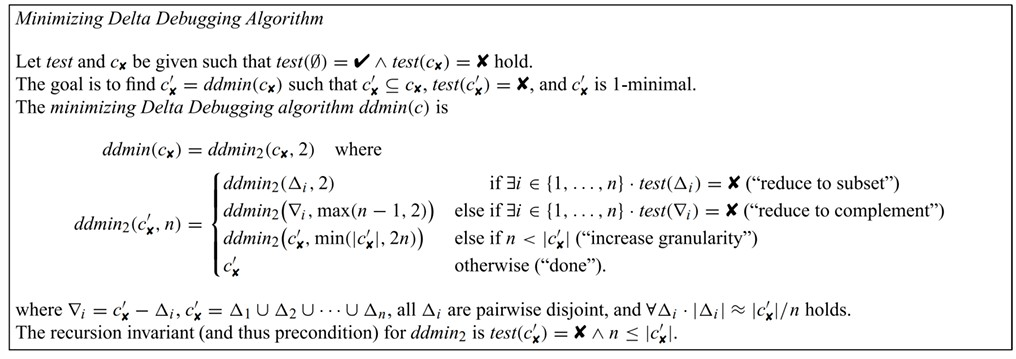
\includegraphics[width=1\linewidth]{deltaDebugging}}

\subsubsection{Delta Debugging PseudoCode}
\begin{lstlisting}
function ddmin(c):
    n = 2
    while len(c) ≥ 2:
        split c into n subsets: Δ1, Δ2, ..., Δn
        for each Δi:
            if test(c - Δi) == FAIL:
                return ddmin(c - Δi)
        for each Δi:
            if test(Δi) == FAIL:
                return ddmin(Δi)
        if n == len(c):
            break
        n = min(len(c), n * 2)
    return c
\end{lstlisting}


\subsubsection{Isolating Failure-Inducing Changes}
\begin{itemize}[itemsep=-1pt]
\item \textbf{Regression Bugs}: Features work in previous versions, fail in newer ones.
\item \textbf{Git Bisect}: Automates the process of identifying the commit that introduced a regression bug using binary search.
	\begin{itemize}
		\item Steps: Mark a known good version (\texttt{git bisect good}) and a bad version (\texttt{git bisect bad}). Test intermediate versions until the first bad commit is identified. Can be automated using scripts that build and test the program for each version.
	\end{itemize}
\item \textbf{Delta Debugging on Changes}: Applies delta debugging to individual patches within a commit. Granularities include hunks (consecutive differing lines) or entire changesets.
\end{itemize}


\subsection{7. \underline{Software Development Practices}}
\textbf{Development Practices}: Asking `How'. Credits: Guest Lecturer Kareem Shehata.

\subsubsection{Source Control Management (SCM)}
\begin{itemize}[itemsep=-1pt]
\item \textbf{Questions to ask}: Who is allowed to view, change code? How are changes managed? dependencies managed? How does source control integrate with tools?
\item \textbf{SCM Tool Considerations}: (source control $\neq$ git!)
	\begin{itemize}
	\item \textbf{Centralized vs Decentralized}: Centralized systems have single repository, decentralized allow multiple repositories w. synchronization.
	\item \textbf{Scalability}: Handle large repositories and teams, \textbf{Development Tool Support}: Integration with IDEs like VS, XCode, \textbf{Expertise/opinions in team}: Choose tools that align with whole team's expertise, preferences. \textbf{Dependency Management}: Tools (Maven, Gradle) help manage deps.
	\end{itemize}
\item \textbf{Good SCM Practices}:
	\begin{itemize}
	\item \textbf{Single Source of Truth}: Maintain single authoritative repository. \textbf{Consistency}: Consistent naming conventions (branches, tags, commits). 	\textbf{Small, Focused Changes}: Commit small, independent changes that are easier to review and revert if necessary. \textbf{Clarity}: Clear commit messages explaining what was changed and why.
	\item \textbf{Use Branches and Tags Appropriately}: Use branches for feature development and tags for releases. \textbf{Avoid Long-Lived Branches}: Merge frequently, reduce integration challenges. \textbf{Use Toolset for Managing Dependencies}: Leverage dependency management tools to handle external libraries.
	\end{itemize}
\end{itemize}

\subsubsection{Coding Style}
Consistent coding style improves readability, maintainability, collaboration. Also, probably need to revisit, read own code in the future.

\begin{itemize}
\item \textbf{Why Care About Style}: Unnecessary changes in SCM due to formatting diff. Inconsistencies make code harder to read, understand. Style differences can lead to confusion and inefficiency.
\item \textbf{Key Elements of a Style Guide}: \textbf{Consistency over Optimality}: Consistency more important than overly optimized code. \textbf{Focus on Clarity}, be clear and unsurprising. \textbf{Practicality over Clever solutions.} Include guidelines on how tasks should be approached, not just formatting rules. \textbf{Autoformatters}: Use tools like Prettier, clang-format, or Black to automate formatting.
\end{itemize}

\subsubsection{Versioning and Releases}
\begin{itemize}
\item \textbf{Releases}: Depends on deploy method. Web services w. rolling releases, app stores, binaries, embed systems will be diff. in deployment, releases.
\item \textbf{Software Versioning}: Process of assigning unique identifiers to bundles of software. Identifiers help track, manage diff releases of software over time. Goals: 
	\begin{itemize}[itemsep=-1pt]
	\item Allow users to know which version of the software using, enable developers to identify version customers are using. 
	\item Managing dependencies between software components.
	\end{itemize}
\end{itemize}

\subsubsection{Semantic Versioning (SemVer)}
Semantic Versioning is a widely adopted versioning scheme, particularly for software with public APIs. It uses a three-part version number: \\ \textbf{MAJOR.MINOR.PATCH}.
\begin{itemize}[itemsep=-1pt]
    \item \textbf{MAJOR version}: Increment: incompatible API changes are made.
    \item \textbf{MINOR version}: Increment: backward-compatible functionality is added.
    \item \textbf{PATCH version}: Increment: backward-compatible bug fixes.
    \item \textbf{Hyrum's Law}: With a sufficient number of users of an API, it does not matter what you promise in the contract: all observable behaviours of your system will be depended on by somebody. 
\end{itemize}
System ensures clarity and consistency in communicating changes to users and devs.  However, these labels are slapped on by a human - no perfect guarantee. 

\subsubsection{Versioning Schemes}
\begin{itemize}
    \item \textbf{Commits as Identifiers}: Source control systems like Git assign unique hashes to commits (e.g., \texttt{2d54f09b}). \textbf{Pros}: Automatic, no additional effort required; useful for internal tracking. \textbf{Cons}: Not all commits correspond to release versions; difficult to remember and interpret.
    \item \textbf{Assigned Identifiers}: Includes code names (e.g., Android's "Lollipop," "Marshmallow") or version increments (e.g., v1, v2, v3).
 Can be combined with tags indicating release stages (e.g., alpha, beta, rc release candidate). \textbf{Pros}: Easier to remember; code names aid branding and communication. \textbf{Cons}: Requires manual assignment and management.
 	\item \textbf{E.g. Versioning in Practice}: \textbf{Android}: Uses both numeric versions and dessert-themed code names (e.g., Android 9: Pie). Code names follow alphabet order, aid in identifying newer versions. \textbf{macOS}: Combines numeric versions with thematic names (e.g., macOS Big Sur, macOS Monterey). \textbf{Ubuntu}: Uses calendar-based versioning (YY.MM) and distinguishes Long-Term Support (LTS) releases.
	\item \textbf{Choosing Versioning Scheme}: Depends on organizational needs, deployment strategies, release frequency, and user expectations. For example: web services with rolling releases may prefer frequent, small increments. Embedded systems/ safety-critical software may strict versioning/ long-term support. (Needs of marketing / users?)
	\item \textbf{Best branching strategy}: Anything that gives a single source of truth, consistent, depends on your organization, deployment strategy, etc!
\end{itemize}
\centerline{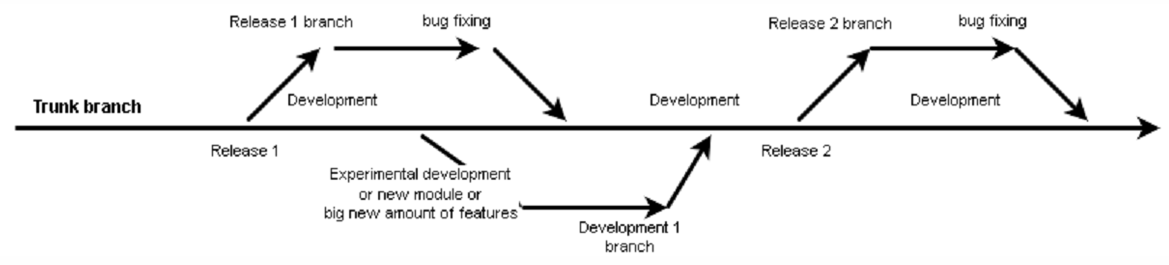
\includegraphics[width=0.8\linewidth]{gitTrunk}}

%\centerline{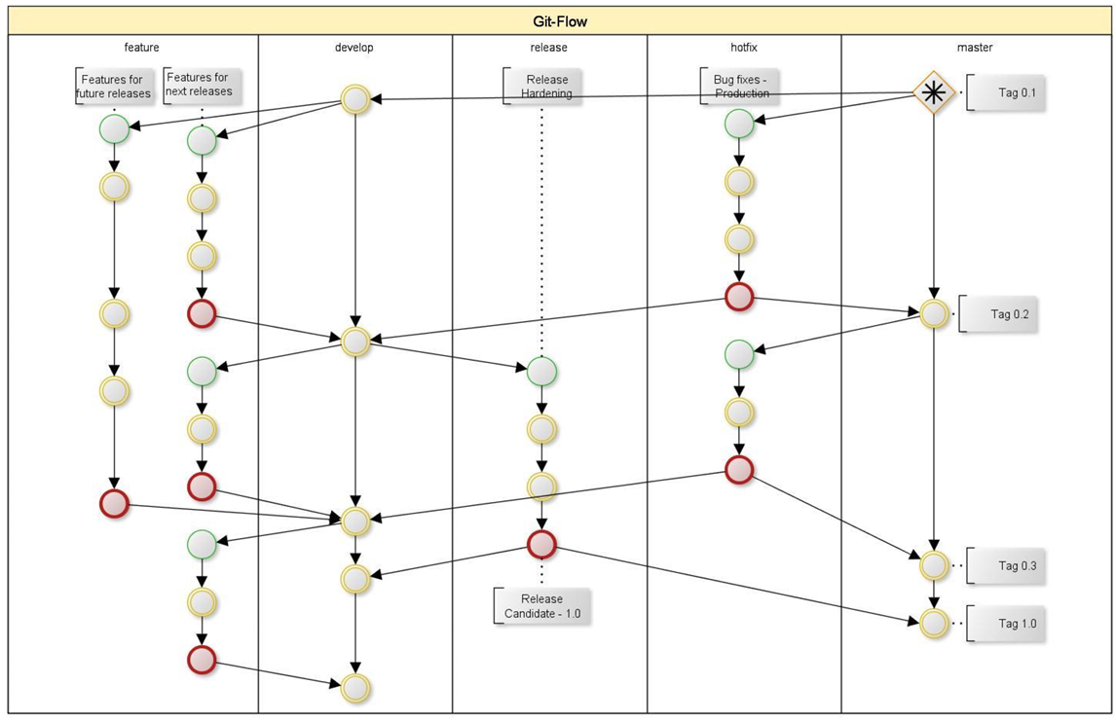
\includegraphics[width=0.5\linewidth]{gitFlow}}

\subsubsection{Dependencies}
Dependencies: external components for software to function correctly, but not directly controlled by development team. Modern software: lot of dependencies!
% \centerline{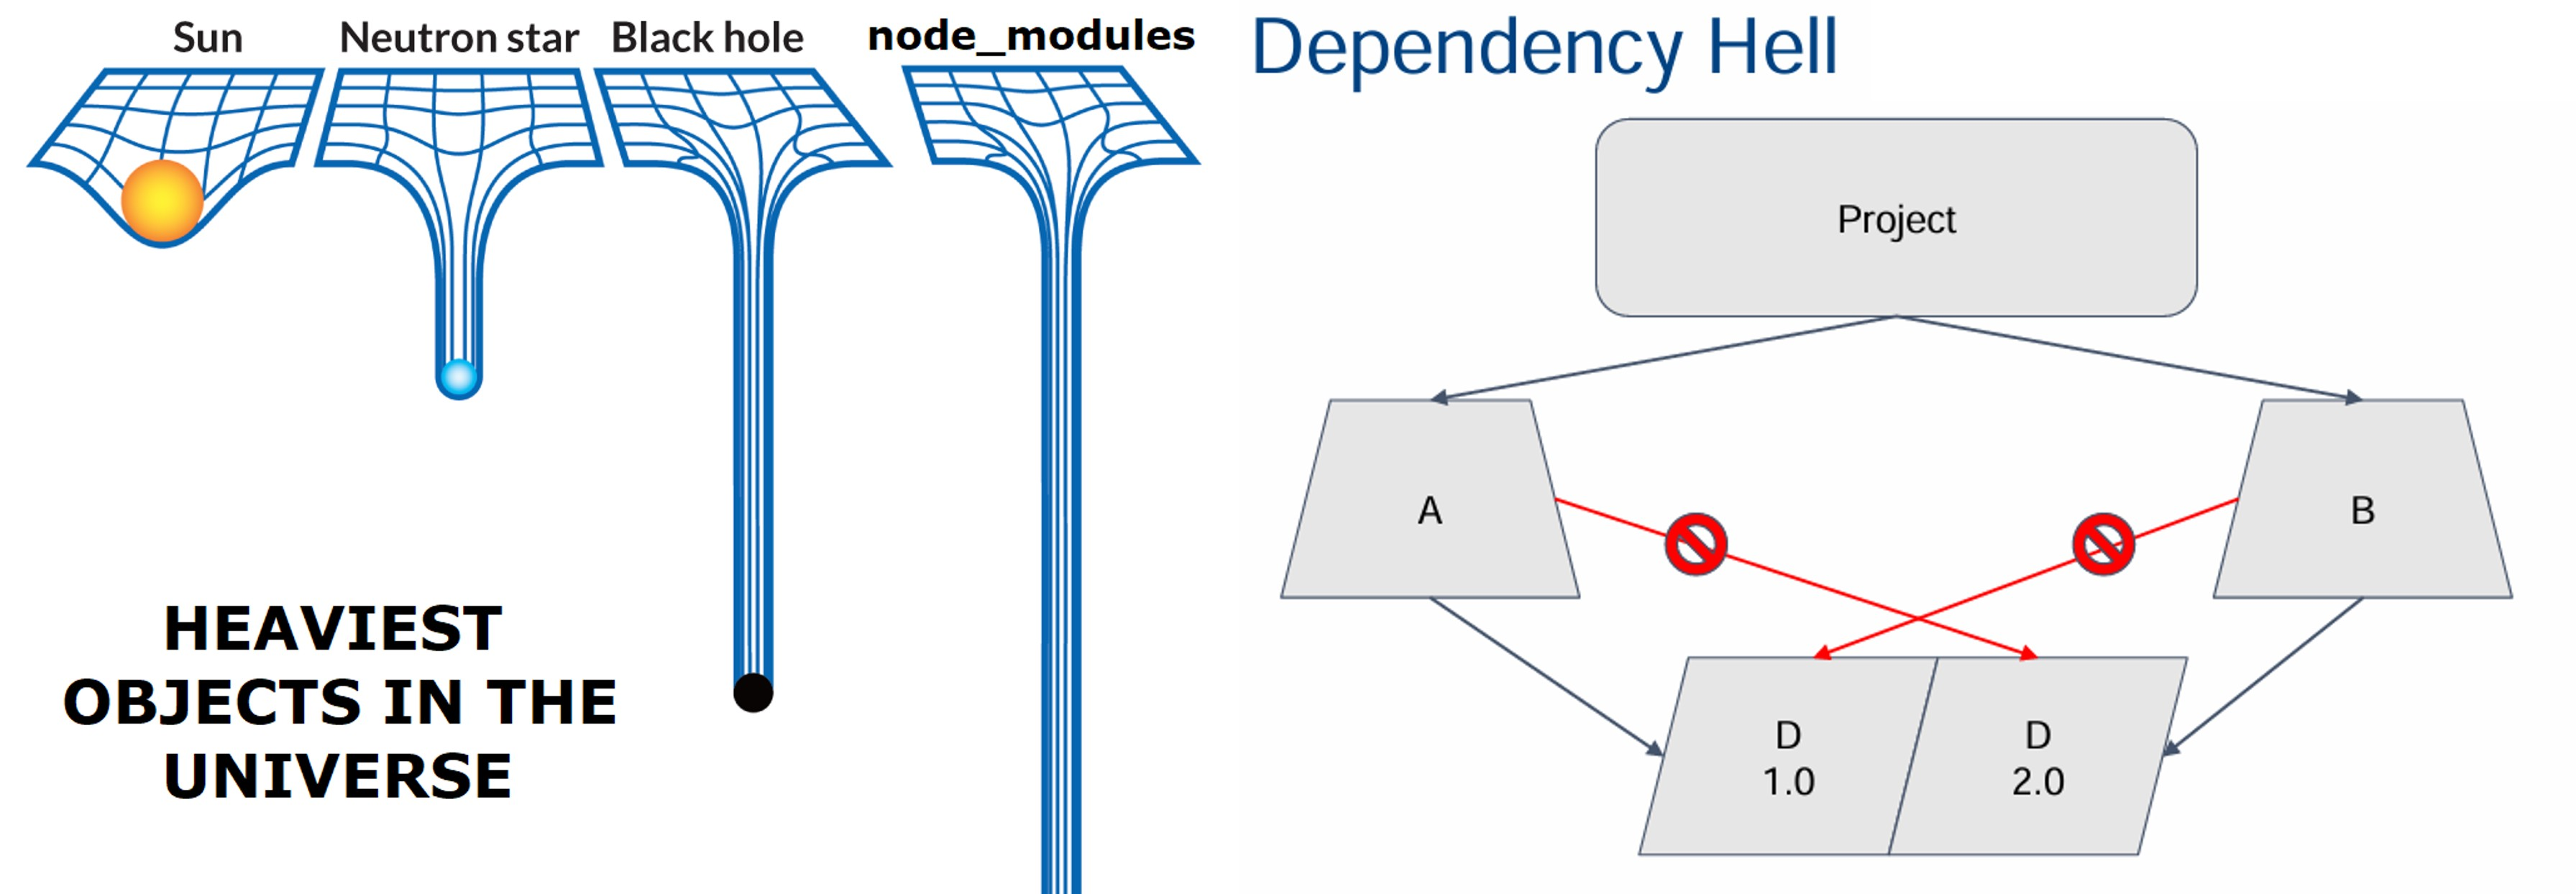
\includegraphics[width=0.9\linewidth]{dependencies}}
\begin{itemize}
    \item \textbf{Examples}: Libraries (e.g., React, TensorFlow), Build tools (e.g., Maven, Gradle), External services (e.g., APIs, cloud platforms).
    \item \textbf{Dependency Hell}: when multiple dependencies conflict, when outdated libraries cause integration issues. Modern software numerous dependencies, increasing complexity of dependency management.
    \begin{itemize}
	\item \textbf{Conflicting versions}: Two deps. require incompatible versions of same library.
	\item \textbf{Circular dependencies}: Packages depend on each other in a loop.
	\item \textbf{Deep dependency chains}: One small update can break many things down the chain.
	\item \textbf{Breaking changes}: Updates in a dependency cause your software to fail.
	\end{itemize}
    \item \textbf{Managing Dependencies} Strategies include: Embedding small or critical libraries directly into project, hosting medium-sized libraries in a private repository, using submodules or package managers for large, well-established libraries. Employing lockfiles and containers to ensure consistent runtime environments.
\end{itemize}

\subsubsection{Deprecation}
Process of orderly migration away from, eventual removal of obsolete systems. Planning, executing a transition strategy to minimize disruption.
\begin{itemize}
    \item \textbf{Why Deprecate?} Code / Dependencies are \textbf{liability, not an asset}. Maintaining outdated systems incurs operational costs. Legacy systems hinder the evolution of newer systems due to compatibility requirements (quote Google). Allows orgs. to focus resources, maintain and improve current systems.
	\item \textbf{Challenges}: Emotional attachment to old systems. Difficulty in funding, executing deprecation efforts. High costs migrating to entirely new systems.
	\item \textbf{Types of Deprecation}: \textbf{Advisory Deprecation}: Inform users about deprecated features without enforcing immediate action. \textbf{Compulsory Depreciation}: Set deadlines for removal and ensure compliance through enforcement.
	\item \textbf{Deprecation During Design}: Design systems with deprecation in mind to simplify future decommissioning. E.g.:
Plan for incremental replacement of components. Ensure clear documentation and migration paths for users (give alternative).
\end{itemize}

\subsubsection{Code Review}
Before deploying new code, critical to ensure quality, correctness. Unreviewed code: lead to bugs, poor design decisions, maintainability issues. Mitigate risks by involving others in process of inspecting, improving code.
\begin{itemize}[itemsep=-1pt]
    \item \textbf{Risk Mitigation}: Code reviews catch defects early, formal reviews identifying up to 60\% of defects (comparatively - 30\% for testing).
    \item \textbf{Maintainability}: Studies: up to 75\% of code review comments address evolvability, maintainability, not just functionality.
    \item \textbf{Other Benefits}: Solicit feedback on code design, practices. Teaching, demonstrating coding methods. Raising awareness of product's state. Highlighting potential future problems.
  	\item \textbf{Challenges}: \textit{Speed vs. Thoroughness}: Review time increases exponentially with the size of the change, leading to diminishing returns on thoroughness. \textit{Balancing Priorities}: if speed or depth of review more important.
\end{itemize}

\subsubsection{Good Practices for Effective Code Reviews}
\begin{itemize}[itemsep=-1pt]
    \item \textbf{Code Review Authors}: Keep reviews small and focused. Clear desc, annotate to guide reviewers. Choose appropriate reviewers, balance feedback quality w. team awareness. Open to feedback, implement suggested changes unless strong reason not. Reflect on feedback to improve future work.
    \item \textbf{Code Reviewers}: Push back on overly broad or poorly described changes. Focus on code, not person. Ask qns, point out problems, suggest solutions. Consider edge cases, failure scenarios, and future maintainability. Be responsive while balancing severity and importance of changes.
\end{itemize}

\subsubsection{Software Quality Assurance (SQA)}
Encompasses all activities aimed at ensuring product quality before reach customers. Unlike testing (finding bugs), SQA addresses broader aspects of quality, including usability, performance, and maintainability.
\begin{itemize}
    \item \textbf{Key Principle}: Just as physical products quality checks, software products to meet high-quality standards before release.
    \item \textbf{SQA Scope}: test, docs, process adherence, customer UX validation.
    \item \textbf{Best Practices}: Simulate real-world customer usage to identify gaps between product, expectations. Ensure QA performed by someone other than developer to avoid biases. Focus on entire customer experience, not just crashes, functional bugs. (E.g. QA engineer tests edge cases (e.g., ordering -1 beers) and unexpected inputs (e.g., "ueicbksjdhd",''where is toilet'').)
\end{itemize}

\subsubsection{Deployment}
Deployment strategy impacts SWE practices. Method of deployment depends on factors e.g. update frequency, scalability, risk tolerance.
\begin{itemize}[itemsep=-1pt]
    \item \textbf{Examples of Deployment Methods}: Zip files on a server, Web apps w. continuous deployment ("DevOps"). App stores (mobile), Physical media (e.g. games), Pre-installed software on devices.
    \item \textbf{Considerations}: Speed, friction for releases/updates. Scalability to handle large user bases. Risks associated with deployment failures. Costs of maintaining infrastructure.
	\item \textbf{Deployment Strategy Examples}: \textit{NASA}: Rigorous testing, version control, minimal runtime dependencies due to limited update opportunities. \textit{Web App}: Allows instant updates, frequent releases, enabling rapid iteration.
\end{itemize}

\subsubsection{Key Takeaways}
\begin{itemize}[itemsep=-1pt]
    \item Learn best practices but adapt them to your organization's needs.
    \item There are no universal solutions; context matters.
    \item Teamwork, collaboration, and consistency outperform individual heroics.
    \item Think critically about organizational priorities when choosing practices.
\end{itemize}

\subsubsection{Differences Between Junior and Senior Developers}
\begin{itemize}
    \item \textbf{Junior Devs}: Hide code until "ready." Provide inaccurate estimates, deliver inconsistently. Use long-lived branches, big merges. Large, unstructured commits w. unclear messages. View code review feedback as criticism.
    \item \textbf{Senior Devs}: Share code, ideas during dev. Provide accurate estimates, deliver on time. Use short-lived branches w. smaller merges. Make small, focused commits w. clear reasoning. View code review feedback as opportunity to improve.
    \item \textbf{Agility in Software Engineering}: "Solutions to common software engineering problems not always obvious. Agility - both technical and organizational - is essential to identify solutions that work for current challenges and remain resilient to future changes." - Asim Husain, VP Eng, Google.
\end{itemize}

% ---------------------
\subsection{8. \underline{Static Analysis and Type System}}


\subsubsection{Limitations of Testing}
\begin{itemize}
\item \textbf{Testing} widely used to identify bugs, but has significant limitations. Demonstrates presence of bugs but cannot guarantee their absence. Often time-consuming and resource-intensive. Edge cases and rare conditions may remain untested.
\item \textbf{Historical Context of Software Failures}: significant financial losses and even endangerment of human lives. E.g. Mars Climate Orbiter (1998), Knight Capital Group (2012) trading glitch loss \$440 million. Wannacry Ransomware Attack (2017). Boeing 737 MAX Crisis (2019).
\item \textbf{Static analysis, type systems} can help play a crucial role in improving software reliability and reducing the incidence of costly bugs (Fewer runtime errors).
\end{itemize}

\subsubsection{Static Analysis}
\begin{itemize}
\item \textbf{Static analysis}: examination of code without executing it. 
\item \textbf{Primary goals}: identifying potential errors, adherence to coding standards, optimizing performance.
\item \textbf{Why Static Analysis}: Early detection of bugs, reduce fix cost later in dev process. Improved code quality by enforcing best practices.
	Reduced debugging time through automated checks. Enhanced maintainability by ensuring consistent coding styles and fewer runtime errors.
\item \textbf{Types of Static Analysis}:
	\begin{itemize}
	\item \textbf{Linters and Style Checkers}: Focus on formatting and adherence to coding conventions without deeper semantic analysis.
	\item \textbf{Data-Flow Analysis}: Tracks the flow of data through a program to determine possible values at different points in the execution.
	\item \textbf{Control-Flow Analysis}: Analyze order of statement/function execution.
	\item \textbf{Type Checking}: Verifies that variables and expressions are used consistently according to their declared types. (Focus on this)
	\end{itemize}
\end{itemize}

\textbf{The Problem with Unsafe Languages}: E.g. Python, C, C++, and JavaScript, are inherently unsafe. These languages attempt to execute programs that may fail at runtime due to type mismatches or other errors.
\begin{itemize}
\item Python evaluates unsafe programs, throw runtime error when issues arise.
\item C and C++ place the burden of writing safe programs entirely on the programmer, often leading to manual errors. (Manual proven uneffective)
\end{itemize}


\subsubsection{Type System, Role in Static Analysis}
\begin{itemize}
\item \textbf{A type system}: tractable syntactic method for proving absence of certain prog. behaviors by classifying phrases according to kinds of values they compute. (Benjamin Pierce, Types and Programming Languages)
\item Type systems serve as critical component of static analysis, detect type-related errors before runtime. A type system acts as a filter.
\item\textbf{Well-Typed Programs}: Adhere to type rules, allowed to execute. (e.g. $0 + 1$)
\item \textbf{Ill-Typed Programs}: Prog w. Type mismatch reject before execution (e.g. $false \; 0$ - cannot apply boolean to integer).
\item \textbf{Benefits of Type Systems}: 
	\begin{itemize}
	\item \textbf{Safety}: Prevents runtime errors caused by type mismatches.
	\item \textbf{Early Error Detection}: Identifies errors during development than runtime.
	\item \textbf{Improved Readability and Maintainability}: Clear type annotations make code easier to understand and modify.
	\end{itemize}
\end{itemize}

\subsection{$\lambda$-Calculus}
\begin{itemize}
\item \textbf{Prog. language} invented in 1930s by Alonzo Church and Stephen Cole Kleene.
\item "Core language" w. essential features to express all computation. (Lambda calculus is Turing complete). No redundancy, encode extra features as `syntactic sugar.'
\item Foundations of functional programming (e.g., Lisp, ML, Haskell).
\item Often used as a core language to study language theories. (Type systems, Scope and binding, Higher-order functions, Denotational semantics, Program equivalence)
\end{itemize}
    

\subsection{Overview: $\lambda$-Calculus as a Language}
\begin{itemize}
\item \textbf{Syntax} (How to write program): Keyword "$\lambda$" for defining functions.
\item \textbf{Semantics} (How to describe execution): \textit{reduction} as calculation rules.
\item \textbf{Main Points About $\lambda$-Calculus}: Succinct function expressions using $\lambda$.Bound variables can be renamed ($\alpha$-equivalence). Reduction via substitution ($\beta$-reduction). Can be extended with: Types (e.g., simply-typed $\lambda$-calculus), and side-effects (not covered here).
\end{itemize}
    
\subsubsection{Syntax}
\begin{itemize}
\item $\lambda$-terms or $\lambda$-expressions: $ \text{(Terms)} \quad M, N ::= x \mid \lambda x. M \mid M N $
\item \textbf{Lambda abstraction}: ($\lambda x.M$): Anonymous functions.
\item  \textbf{Lambda application}: ($M N$). 
\item \textbf{Pure/Extended $\lambda$-Calculus}: Pure $\lambda$-calculus only has $\lambda$-terms. Extended has added extra operations and data types. (E.g. $\lambda x. (x + 1), \quad \lambda z. (x + 2y + z)$)
\item \textbf{Conventions (Associativity)}
	\begin{itemize}
	\item \textbf{Body of $\lambda$ extends as far to the right as possible}: \\
	$\lambda x. M N \quad \text{means} \quad \lambda x. (M N), \quad \text{not} \quad (\lambda x. M) N$
	\item \textbf{Function applications are left-associative}: \\
	$M N P \quad \text{means} \quad (M N) P, \quad \text{not} \quad M (N P) $
	\item Examples: \\
	$(\lambda x. \lambda y. x - y) 5 3 \quad = \quad ((\lambda x. \lambda y. x - y) 5) 3$ \\
	$(\lambda f. \lambda x. f x) (\lambda x. x + 1) 2 \quad = \quad ((\lambda f. \lambda x. f x) (\lambda x. x + 1)) 2$
	\end{itemize}
\end{itemize}

\subsubsection{Higher-Order Functions}
\begin{itemize}
\item Functions as \textbf{return values}: $\lambda x. \lambda y. x - y$
\item Functions as \textbf{arguments}: $(\lambda f. \lambda x. f x) (\lambda x. x + 1) 2$
\item \textbf{Example}: Function Composition: \\
Given function $f$, return function $f \circ f: \quad \lambda f. \lambda x. f (f x)$
\end{itemize}
\centerline{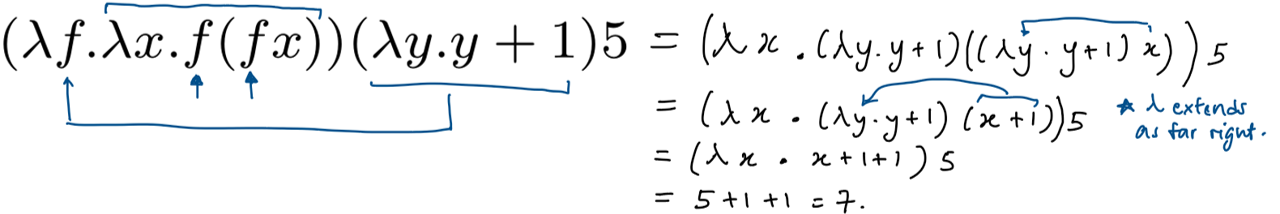
\includegraphics[width=0.7\linewidth]{HOF}}

\subsubsection{Curried Functions}
\begin{itemize}
\item $\lambda$ abstraction is a function of one parameter.
\item $\lambda x. \lambda y. x - y \quad \leftrightarrow \texttt{int f(int x, int y) \{ return x - y; \}}$: \\
Computationally equivalent (can be transformed into each other).
\item \textbf{Curry}: Transform $(\lambda (x, y). x - y)$ to $(\lambda x. \lambda y. x - y)$. Uncurry: Reverse of Curry.
\end{itemize}

\subsubsection{Free and Bound Variables}
\begin{itemize}
\item E.g. $\lambda x. x + y$. $x$: Bound variable. $y$: Free variable.
\item Bound variables renameable ($\alpha$-equivalence): $\lambda x. (x + y) \Leftrightarrow  \lambda z. (z + y)$
\item Name of free variables matters: $\lambda x. (x + y) \neq \lambda x. (x + z)$
\item \textbf{Occurrences}: $ (\lambda \underline{x. x} + y) (x + 1):$ $x$ has both free and \underline{bound} occurrence.
\end{itemize}
    
\subsection{Processes in Lambda Calculus}
\begin{enumerate}
\item \textbf{Alpha Conversion}: If are applying two lambda expressions w. same variable name inside, change one of them to a new variable name. E.g. 
$(\lambda x.xx)(\lambda x.x) \rightarrow  (\lambda x.xx)(\lambda y.y)$
\item \textbf{Beta Reduction (Basically Substitution)}: Process of calling lambda expression with input, and getting output. E.g. $(\lambda x.xy)z \implies zy$.
Substitution: $(\lambda x. M) N \to M[N/x] $. (`N replaces x in M'). Repeatedly apply the reduction rule to any sub-term. 
\item \textbf{Eta Conversion/Eta Reduction}: Special case reduction. Converts between $\lambda x.(f x)$ and $f$ whenever $x$ does not appear free in $f$. Basically means $\lambda x.(f x) = f$ if $f$ does not make use of $x$. E.g. $(\lambda x.(\lambda y.yy)x) = (\lambda y.yy)$
\end{enumerate}


\subsection{Formal Definitions}
\textbf{Terms}:
    \[
    M, N ::= x \mid \lambda x. M \mid M N
    \]
\begin{itemize}
\item \textbf{Set of free variables} in $M$: $fv(M)$
    \[
    fv(x) \coloneqq \{x\}, \quad fv(\lambda x. M) \coloneqq fv(M) \setminus \{x\}, \quad fv(M N) \coloneqq fv(M) \cup fv(N)
    \]
E.g.: $fv((\lambda x. x) x) = \{x\}, \quad fv((\lambda x. x + y) x) = \{x, y\}$

\item \textbf{Substitution}: Only replace free variables.
\[ M[N/x]: N \text{ replaces } x \text{ in } M \]
Substitution – Avoid Name Capture. Rename bound variables before substitution:
        \[
        (\lambda x. x - y)[x/y] = (\lambda z. z - y)[x/y] = \lambda z. z - x
        \]
\item \textbf{Alpha-equivalence}: $\lambda x. M = \lambda y. M[y/x], \quad \text{where } y \text{ is fresh.}$. Two terms are $\alpha$-equivalent iff one convertable to other purely by renaming bound variables.
\item \textbf{Beta-reduction} (substitution): $(\lambda x. M) N \to M[N/x] $. (`N replaces x in M'). \\
Repeatedly apply the reduction rule to any sub-term.
\end{itemize}

\subsubsection{Normal Form}
\begin{itemize}
\item \textbf{\underline{Red}ucible \underline{Ex}pression} ($\beta$-redex): A term of the form $(\lambda x. M) N$.
\item $\beta$-normal form: A term containing no $\beta$-redex. 
\item Stopping point: Cannot further apply $\beta$-reduction rules. \\
\centerline{ E.g. $(\lambda f. \lambda x. f (f x)) (\lambda y. y + 1) 2 \to 2 + 1 + 1 \quad (\beta\text{-normal form})$}
 Can further reduce to $4$ if reduction rules for $+$ are defined.
 \item E.g.: $\lambda x. \lambda y. x$ (normal), $(\lambda x. \lambda y. x) (\lambda z. z)$ and $\lambda x. (\lambda y. x) (\lambda z. z)$ (not normal)
\end{itemize}

\subsubsection{Confluence (Church-Rosser Property)}
\begin{itemize}
\item Terms can be evaluated in any order. Final result (if exists) is uniquely determined.
\item `When applying reduction rules to terms, the ordering in which the reductions are chosen does not make a difference to the eventual result.'
\item \textbf{Confluence Theorem}: $\text{For all } M, M_1, M_2, \text{ if } M \to^* M_1 \text{ and } M \to^* M_2, \text{ then } \exists M' \text{ such that } M_1 \to^* M' \text{ and } M_2 \to^* M'.$
\end{itemize}

\subsubsection{Non-Terminating Reduction}
\begin{itemize}
\item Some terms have no normal forms. 
\item E.g. $(\lambda x. x x) (\lambda x. x x) \to (\lambda x. x x) (\lambda x. x x) \to \dots$
\item Term may have both terminating and non terminating reduction sequences.
\end{itemize}

\subsection{Reduction Strategies}
\begin{itemize}
\item \textbf{Normal-order reduction}: Choose the left-most, outer-most redex first.
    \[
    (\lambda u. \lambda v. v) ((\lambda x. x x)(\lambda x. x x)) \to \lambda v. v
    \]
\item Normal-order reduction will find a normal form if it exists.
\item \textbf{Applicative-order reduction}: Choose the left-most, inner-most redex first.
\[
    (\lambda u. \lambda v. v) ((\lambda x. x x)(\lambda x. x x)) \to (\lambda u. \lambda v. v) ((\lambda x. x x)(\lambda x. x x)) \to \dots
    \]
\end{itemize}

% \centerline{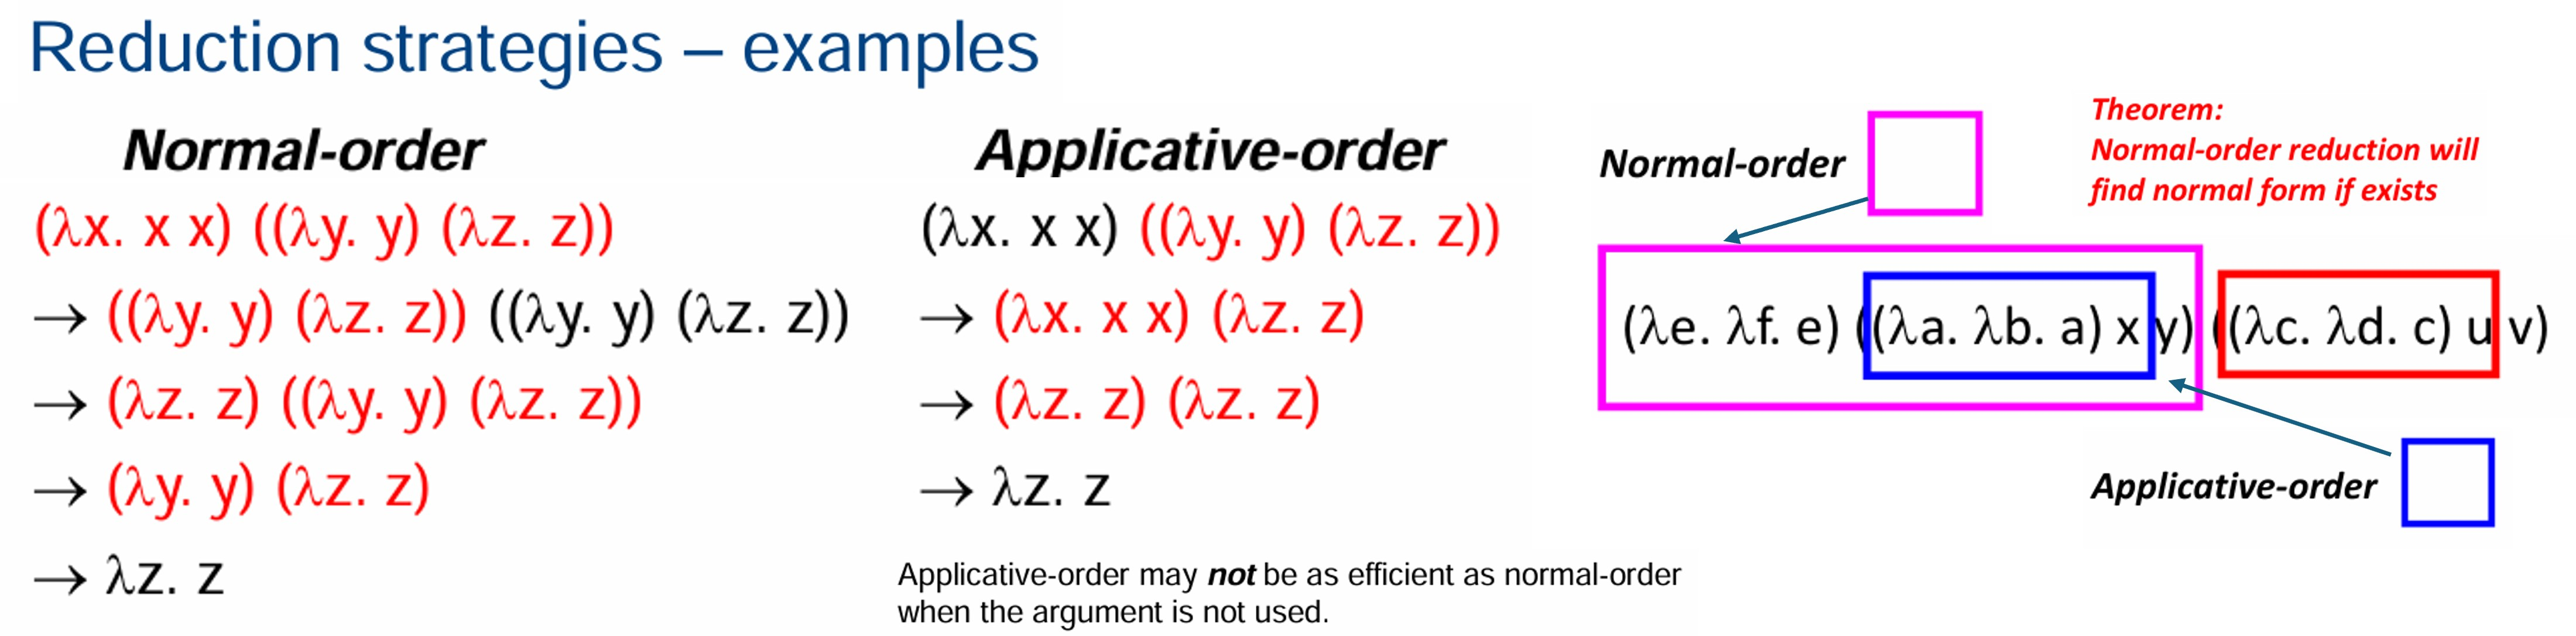
\includegraphics[width=1\linewidth]{reductionStrategies}}

\centerline{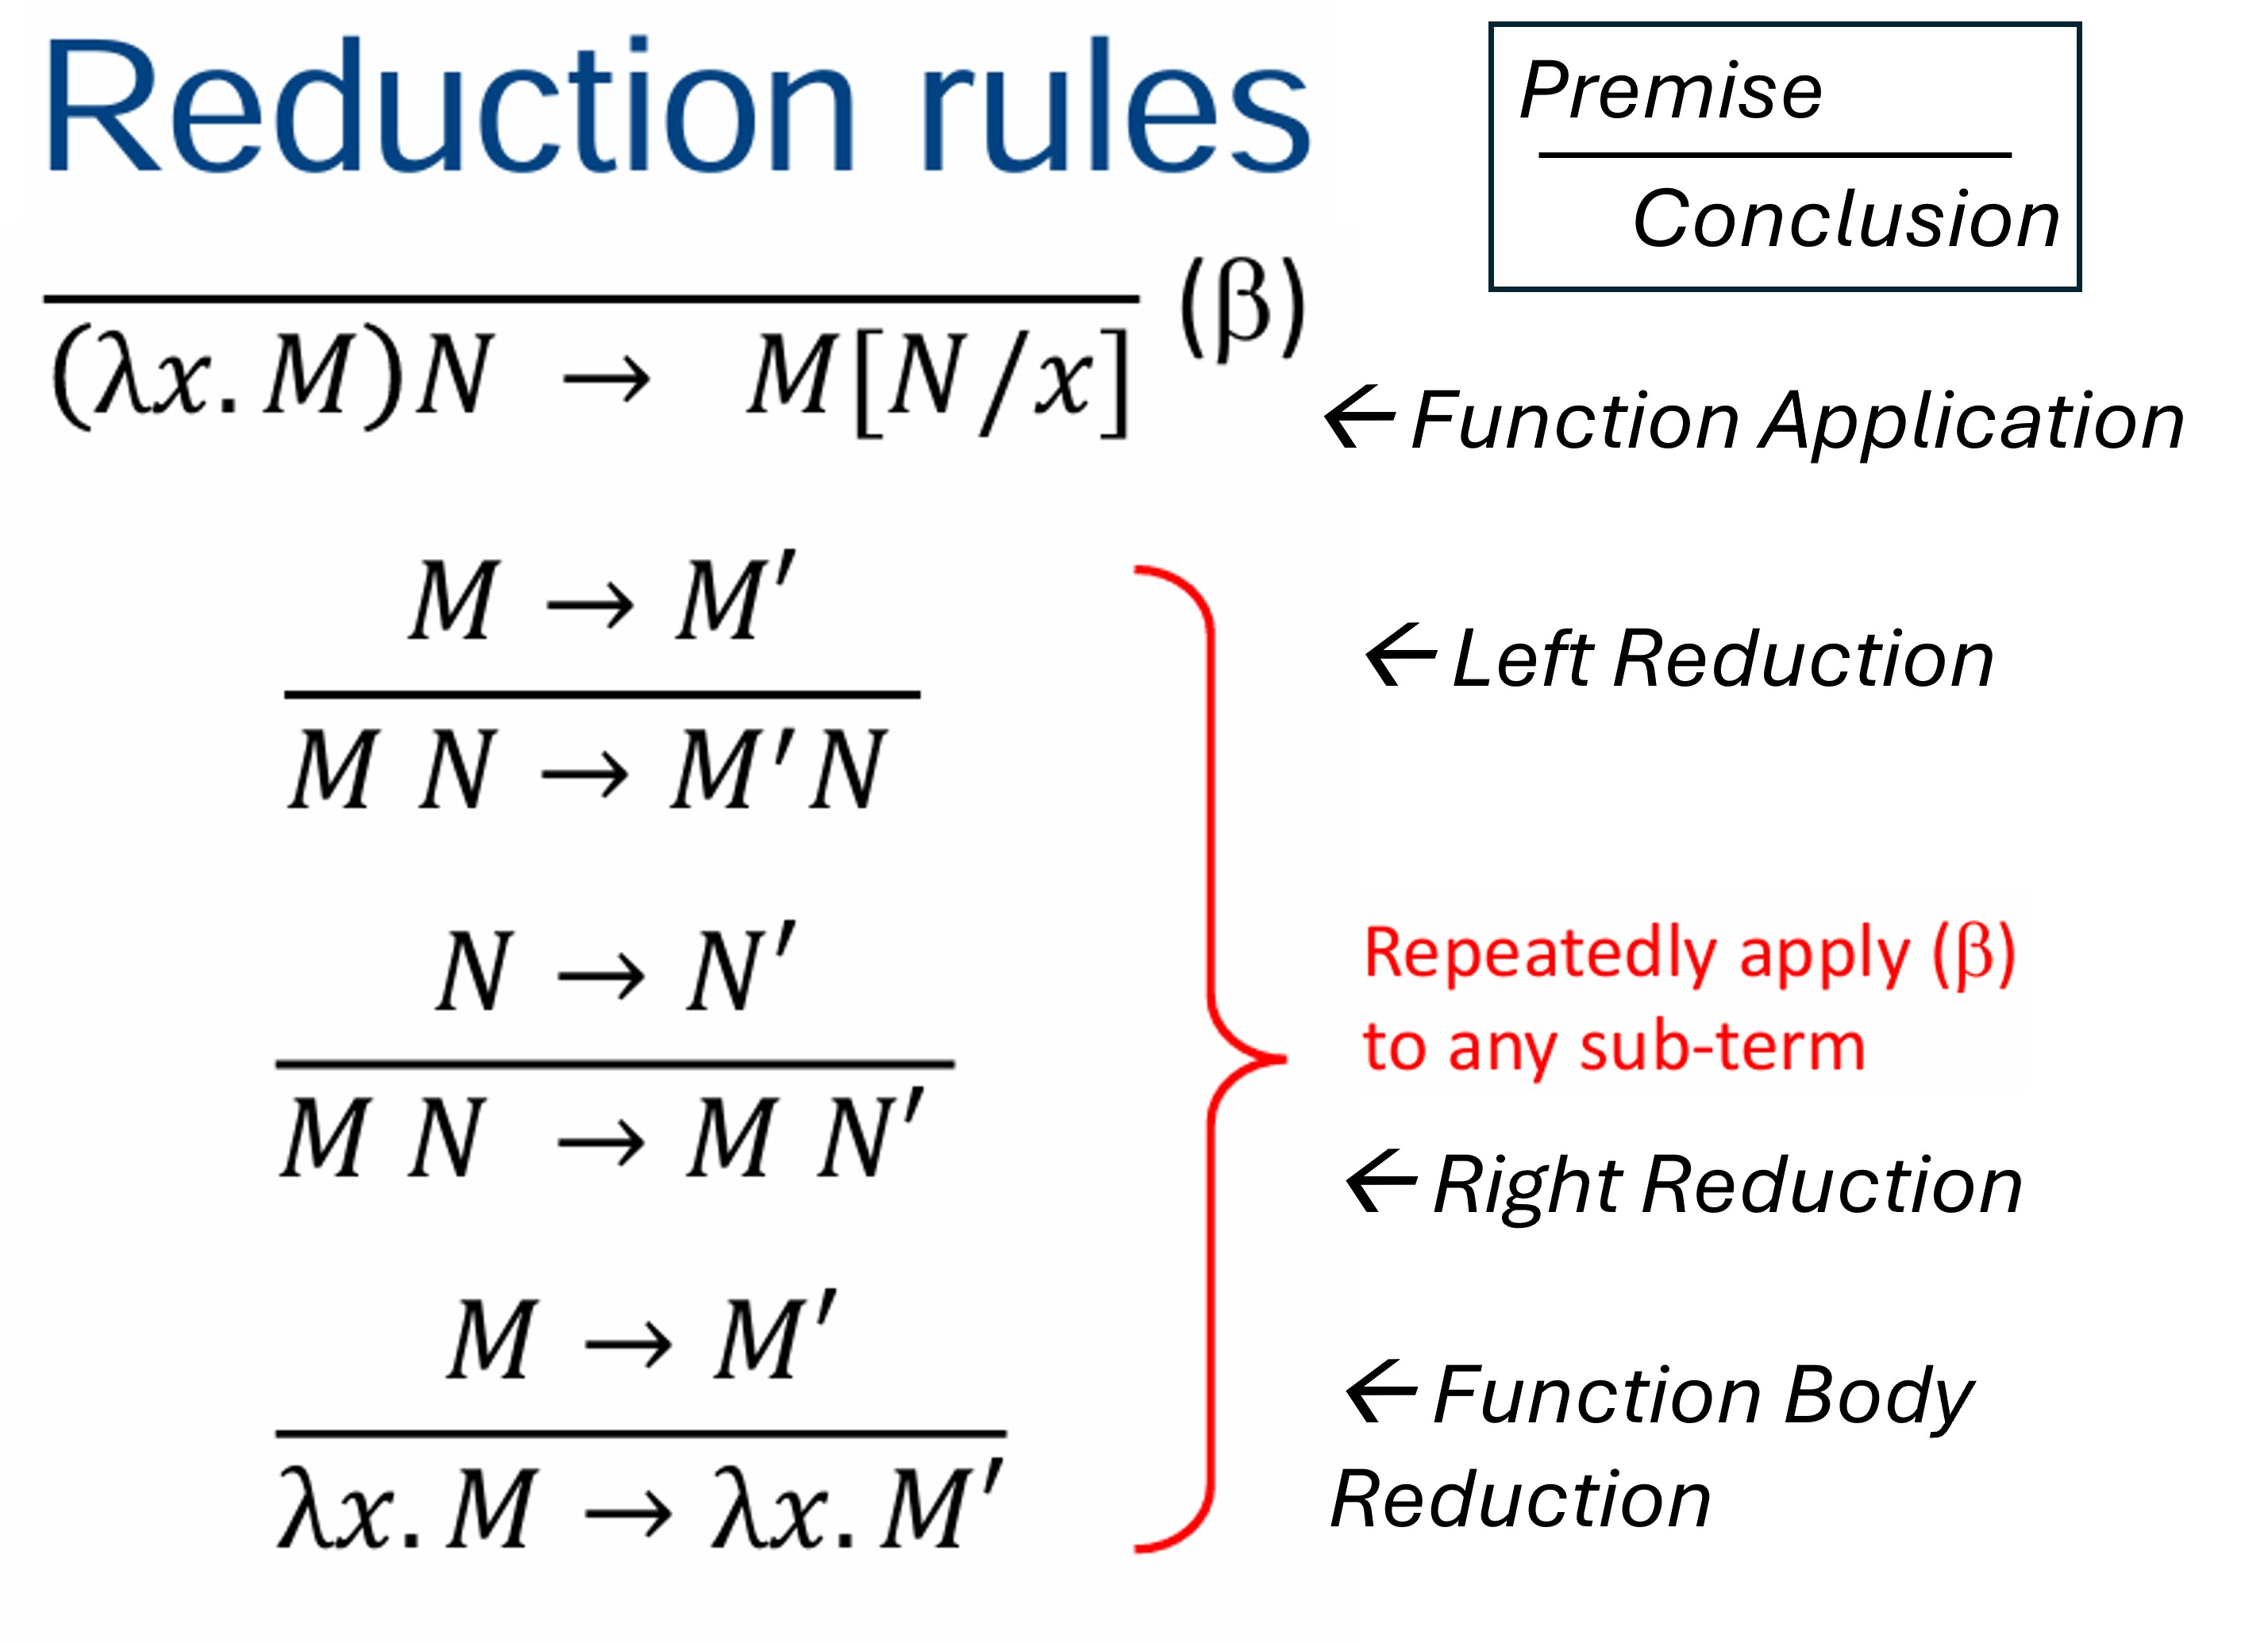
\includegraphics[width=1\linewidth]{reductionRules}}
%\centerline{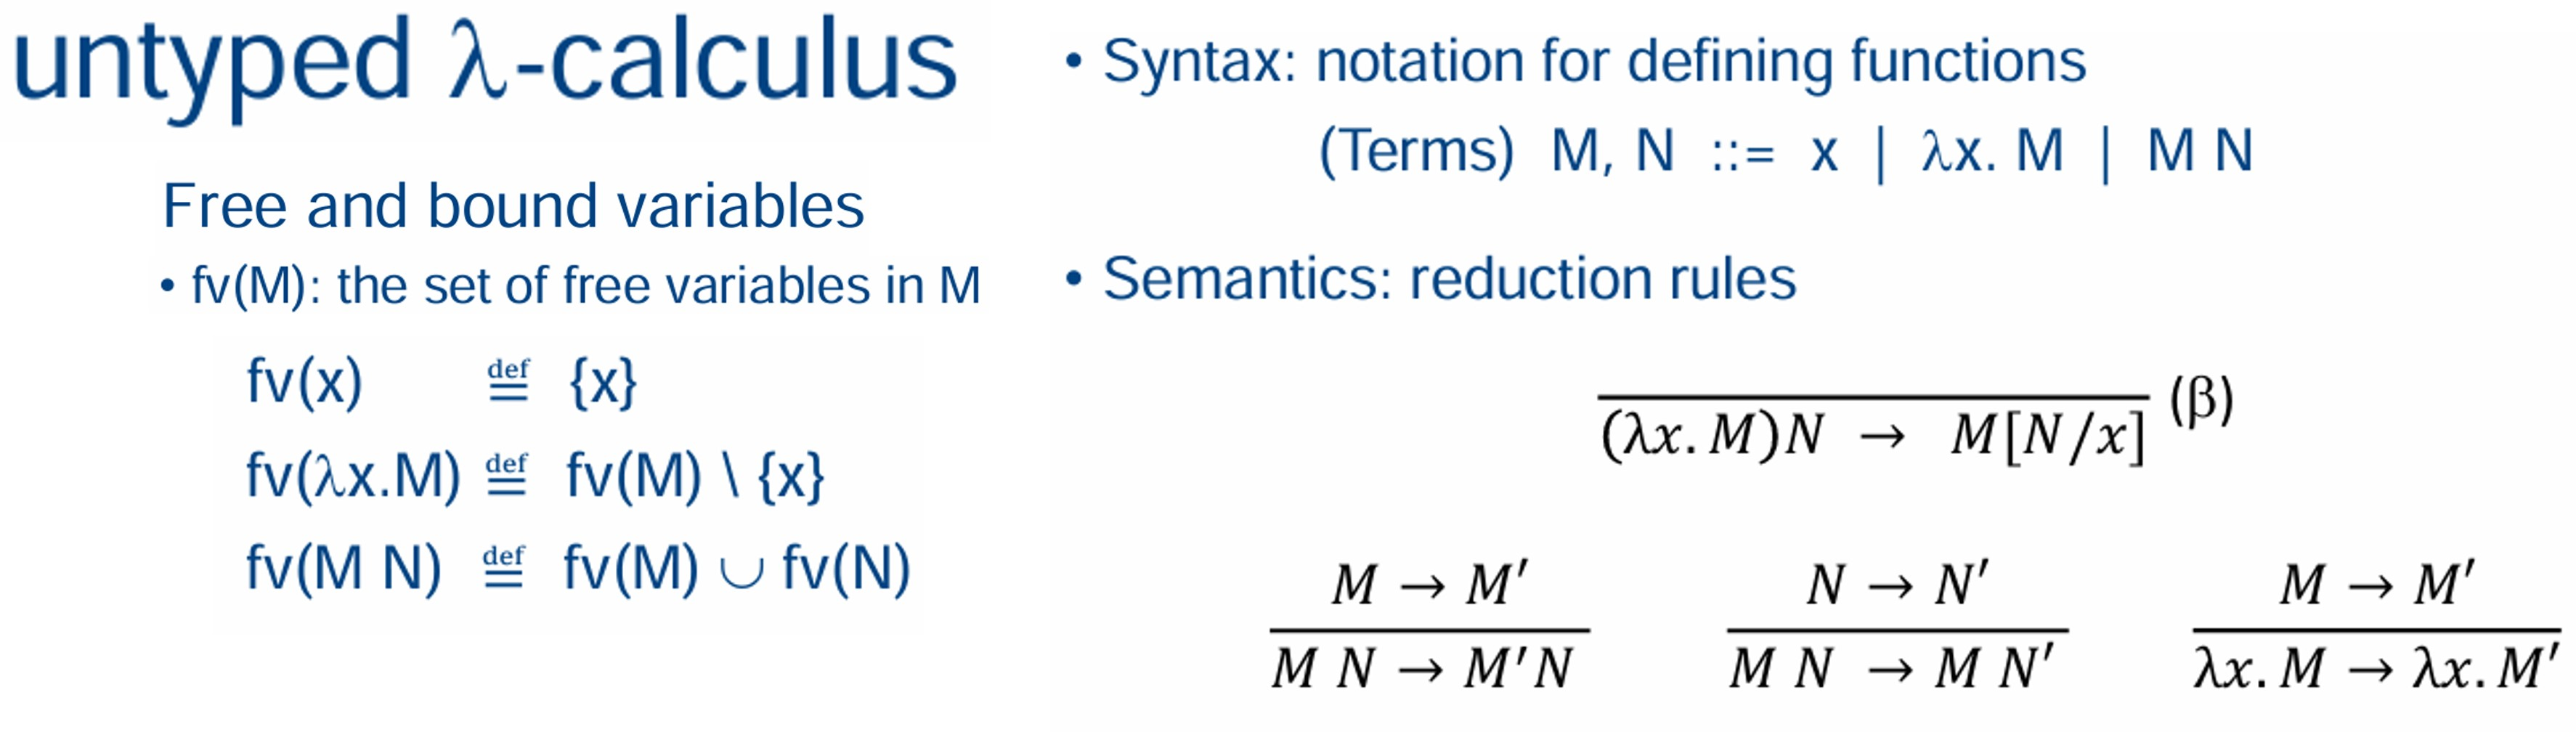
\includegraphics[width=1\linewidth]{untypedLambdaCalculus}}


% \centerline{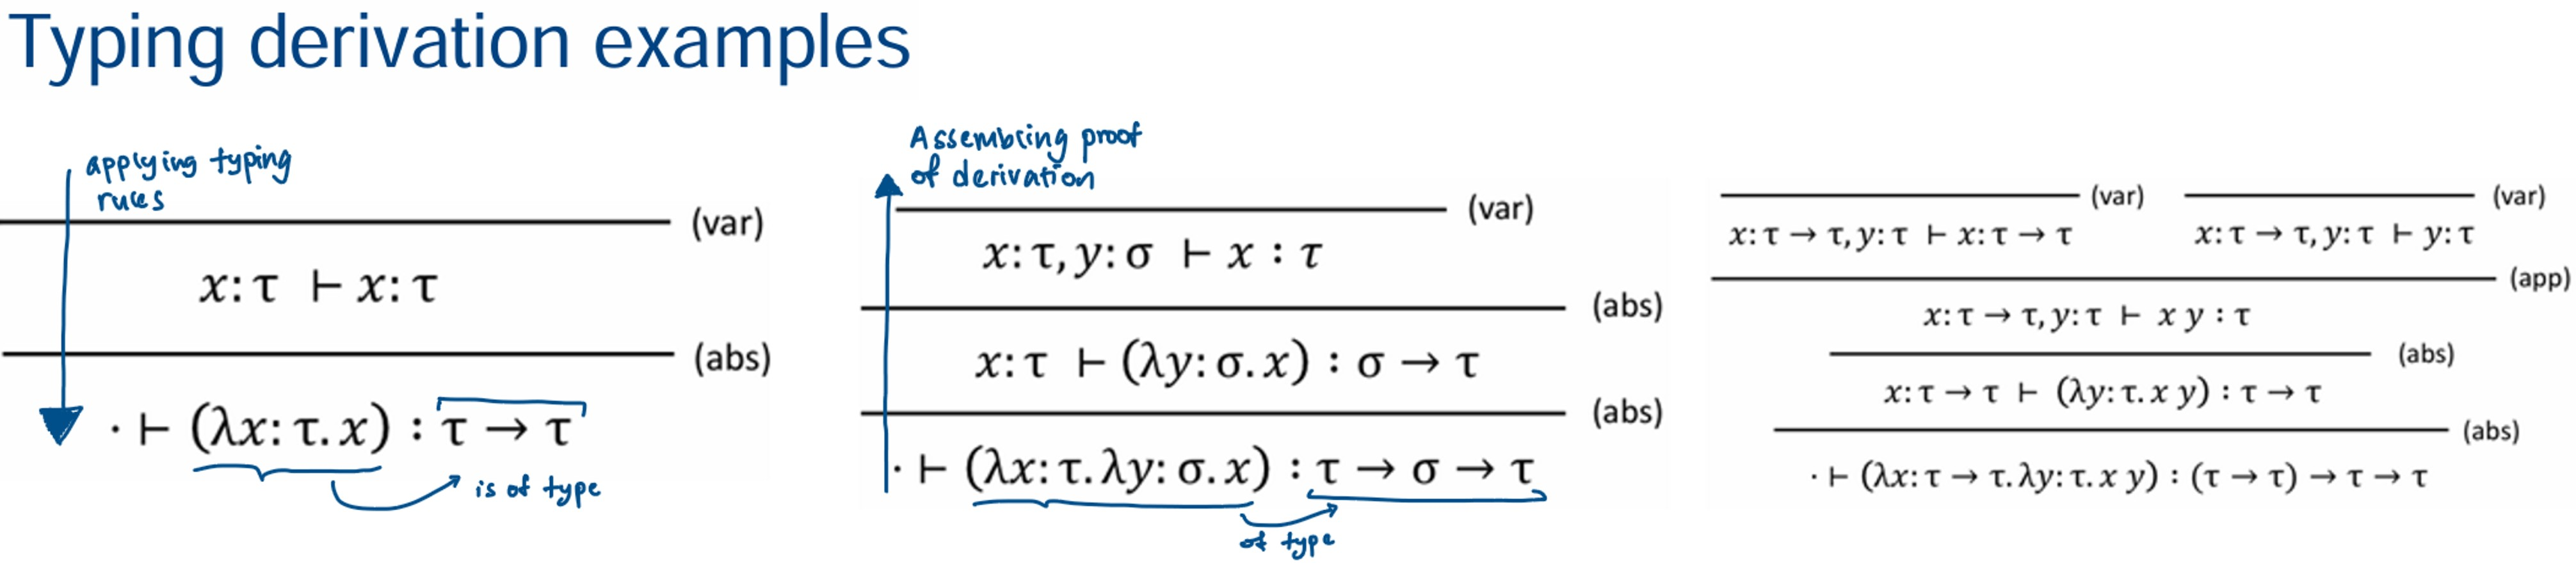
\includegraphics[width=1\linewidth]{typingDerivations}}

\subsubsection{Soundness and Completeness}
\begin{itemize}
\item \textbf{Soundness}: A sound type system never accepts a program that can `go wrong.' Prevents false positives: The language is type-safe. Ensures execution never reaches a "meaningless" state.
\item \textbf{Completeness}: A complete type system never rejects a program that cannot go wrong. Prevents false negatives.
\item In practice, prioritize soundness, minimize false positives. (Impoosible for both)
\end{itemize}
 
% \centerline{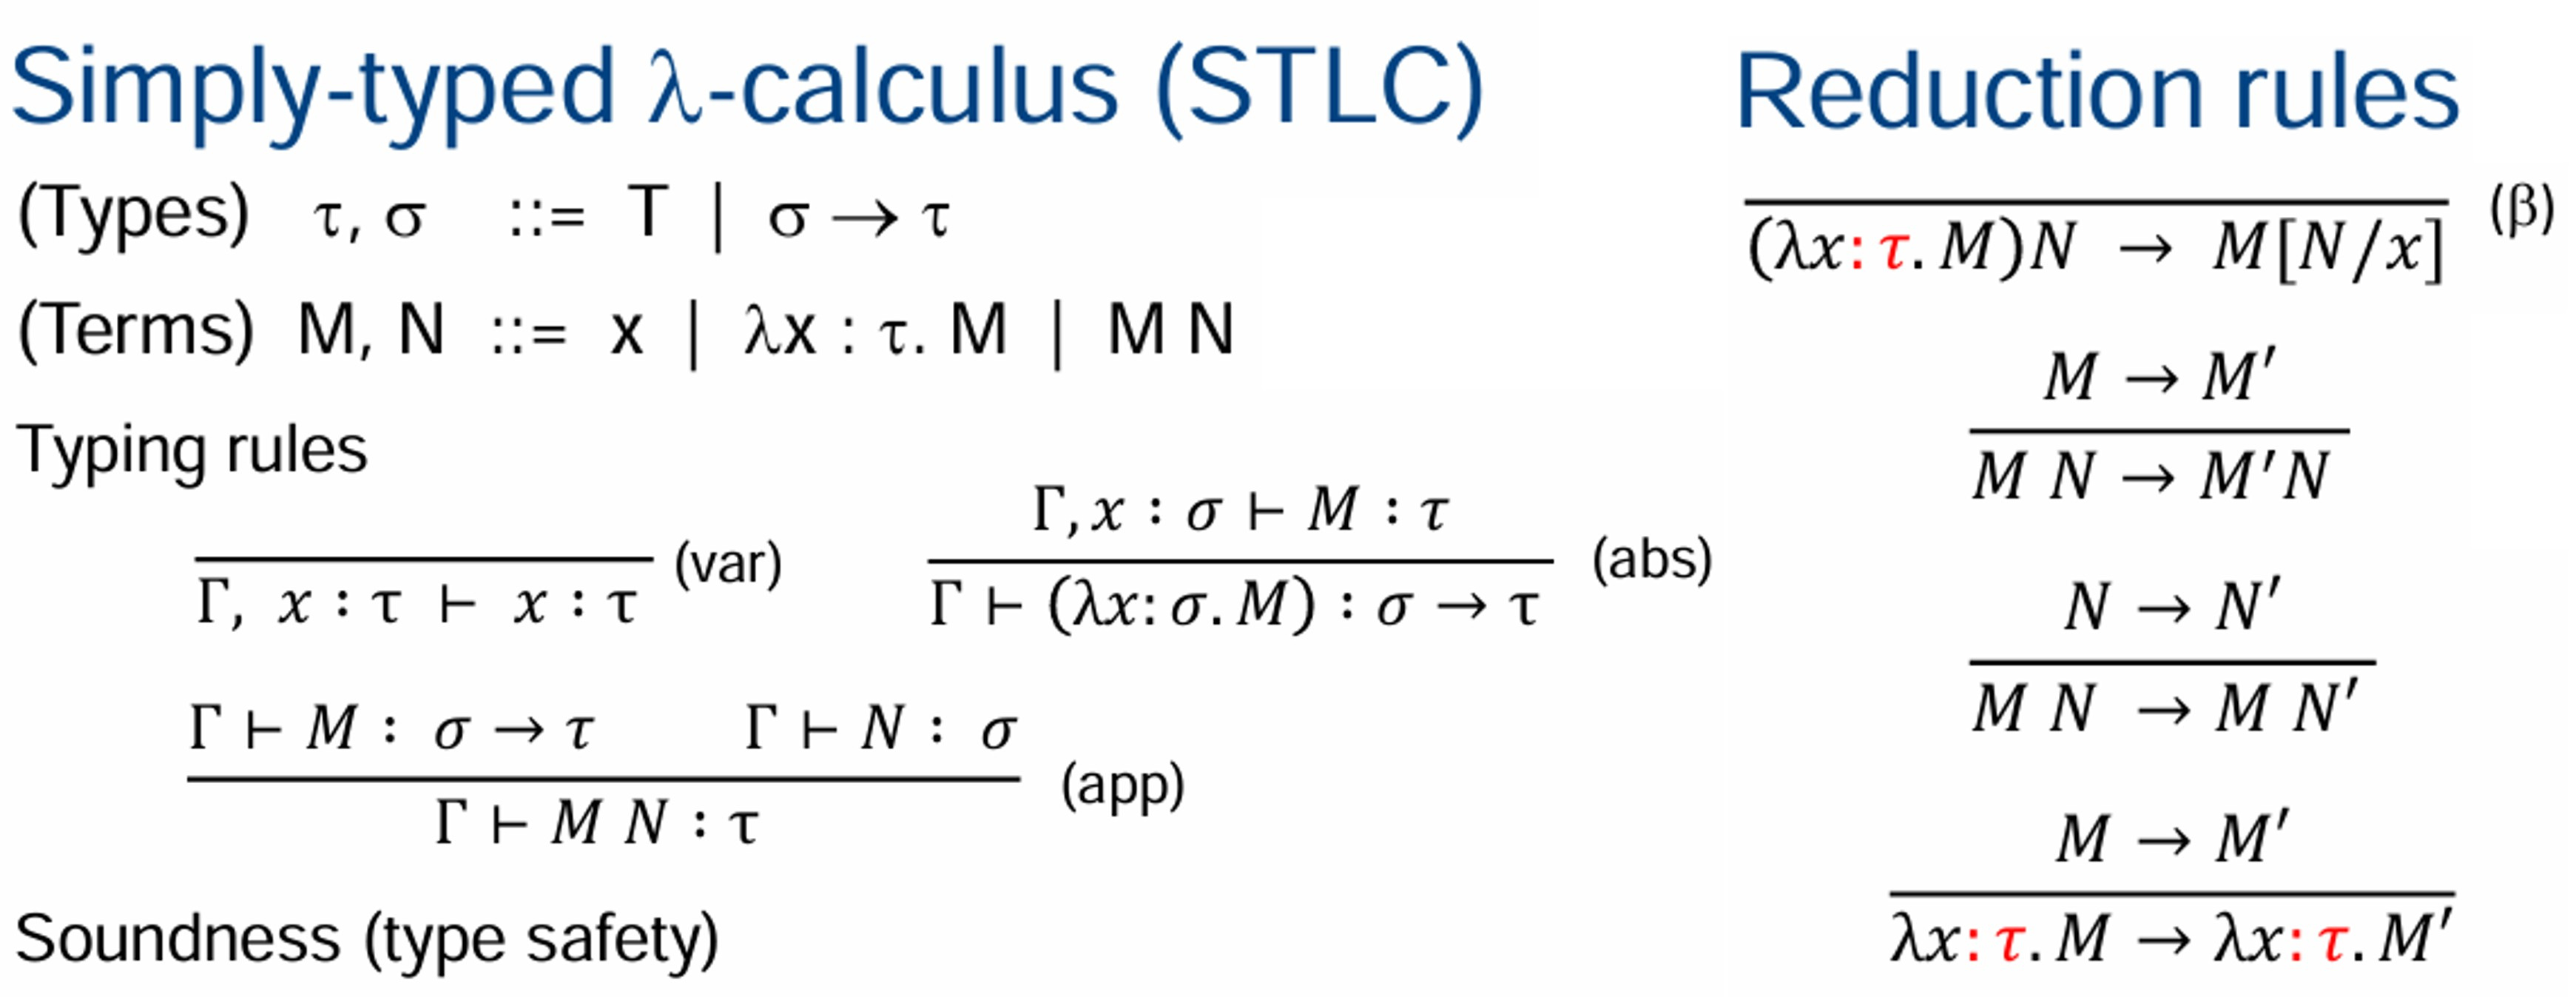
\includegraphics[width=1\linewidth]{STLC}}


% ---------------------------------------------------------------
\subsection{9. \underline{Static Analysis and Type System}}

\subsection{Static Analysis: A High-Level Perspective}
Static analysis involves reasoning about code without executing it. Techniques:
\begin{itemize}
\item \textbf{Type Checkers}: Ensure variables used consistently w. declared types (Topic 8).
\item \textbf{Linters and Style Checkers}: Enforce coding standards, formatting violations.
\item \textbf{Data-Flow Analysis}: Tracks flow of data through program to identify issues.
\item \textbf{Control-Flow Analysis}: Analyzes the possible execution paths of a program.
\end{itemize}
\textbf{Static Analysis Tools in Practice}:  tools developed to detect style violations, potential bugs. E.g. \textbf{Java SpotBugs} (common bug patterns), \textbf{PMD} (code quality, e.g. overly complex methods, unused variables). Tools often face challenges such as false positives, false negatives, integration difficulties.
    

\subsubsection{Soundness vs. Completeness in Static Analysis}
\begin{itemize}
\item \textbf{Soundness}: If tool reports an issue, guaranteed to be true (no false positives).
\item \textbf{Completeness}: If an issue exists, the tool will always report it (no false negatives).
\end{itemize}
Static analysis tools balance the two key properties. Achieving both is undecidable (no algorithm can definitively determine a "yes" or "no" answer for all possible inputs) in practice, leading to trade-offs between the two.

\subsubsection{Challenges with Static Analysis}
E.g. slow execution times, false positives (incorrectly flagged issues) and false negatives (missed bugs), limited applicability to complex features, unactionable warnings, lacking guidance for resolution, difficulty integrating into workflow: 
\begin{itemize}
\item  \textbf{Facebook's Infer Deployment}: Initial deployment, running Infer nightly 2,500 alarms ignored by devs due to workflow disruptions. Integrating Infer during code reviews (on diffs) increased fix rates to over 70\%.
\item \textbf{Google's FindBugs Deployment}: Bug dashboard outside workflows not used. Manually filed bug reports only 16\% fixed. Lastly, integrated FindBugs in code reviews improved adoption but had false positives and inconsistent views.
\item \textbf{Timeliness of reports} crucial; reports addressed when integrated into current tasks. Reporting new issues (on diffs) reduces noise, improve responsiveness.
\end{itemize}

\subsubsection{Key Principles for Successful Static Analysis}
To maximize the effectiveness of static analysis:
\begin{itemize}
\item Focus on developer happiness, ensure understandable, actionable outputs.
\item Maintain low false positive rate (less than 10\%) to build trust in the tool.
\item Integrate seamlessly into developers' workflows (e.g., during code reviews).
\item Provide timely feedback to ensure relevance to the current task.
\end{itemize}



\subsection{Automated Testing {\scriptsize (Auto generate test input, and/or auto apply oracle)}}

\begin{itemize}
\item Automated testing is preferred for complex systems (E.g. OS, compilers, DBMS), as manually written tests may miss bugs or may be incomplete.
\item Example-based testing simpler but less comprehensive than property-based testing.
\item \textbf{Black, Grey, White-box Approaches}: No standard definition
	\begin{itemize}
	\item Black-box: no internal information (e.g., works on the binary only)
	\item White-box: internal information (systematically analyze program)
	\item Grey-box: some internal information (e.g., coverage)
	\end{itemize}
\end{itemize}

\subsection{Automated Testing: Property-Based Testing}
Property-based testing involves specifying properties that the system should satisfy. The testing framework generates test inputs to check if these properties hold. (Test framework tries to find counterexample to break property / falsify it).

\begin{itemize}
\item \textbf{Example Property}: For a function $ \texttt{Math.abs(x)} $, the property is $ |x| \geq 0 $. (Using jqwik, java property based testing framework).
\begin{verbatim}
@Property
void positiveAbs(@ForAll int val) {
    assertTrue(Math.abs(val) >= 0);
}
// arg0: -2147483648 is input that falsifies property.
\end{verbatim}
\item \textbf{Advantages}: Provides greater confidence than example-based unit tests. Useful for communicating specifications.
\item \textbf{Challenges}: Requires creativity to define meaningful properties.
\item Property based testing frameworks also allow constraining of input domain. Also provide ways to adapt existing generators or create new ones. Also provide shrinkers (test-input reduction tools).
\item \textbf{In practice}: used primarily for testing components of complex systems.  Especially in `high-leverage'
scenarios, where properties are easy to identify and test. 
\item \textbf{E.g.}: Google Translate, properties include round-trip translation similarity, idempotency (output deterministic same result for same input), word count etc.
\end{itemize}

\subsection{Automated Testing: Differential Testing}
Differential testing compares outputs from multiple implementations or versions of the same functionality, or a simple reference engine, to detect discrepancies.
\begin{itemize}
\item \textbf{Approach}: Common input, compare outputs of diff. versions, configurations, or implementations. If outputs differ, at least one system may be affected by bug.
\item \textbf{Comparing Versions}: Check behavior against known-working base version (`golden version'), form of regression testing. Though change might be intended.
\item \textbf{Comparing Configurations}: E.g. different optimization levels, different engines.
\item \textbf{Comparing against Reference Engine}: E.g. mocked component.
\item \textbf{Comparing Implementations}: For many important software systems, multiple (competing 
implementations exist).  If sufficiently similar, they can be used for differential testing. (E.g. DB engines, XML processors, compilers.)
\item \textbf{Challenges}: Small overlap in functionality between system can produce false alarms, may miss out common bugs (e.g. stem from common library used).
\end{itemize}

\subsection{Automated Testing: Metamorphic Testing}
Use source test case and its result to generate \textbf{follow-up test cases}, where differential testing might be inapplicable. Rely on \textbf{metamorphic relations} to infer expected results. Special case of property based testing. Black box approach.

\begin{itemize}
\item \textbf{Example Metamorphic Relation}: $ \sin(\pi - x) = \sin(x) $. Test both $0.5$, $\pi - 0.5$.
\item E.g.  Test a sorting function whether relative order of sorted elements maintained when an element is removed from an input array. First result acts as oracle for second result.
\item E.g. EMI (Equivalence Modulo Inputs) for Compiler testing, create programs that are equivalent only for a given input. Mutate unexecuted part of program running input I, and check if same output for I. Finds bugs as compiler optimizes across both executed and unexecuted parts.
\item \textbf{Strengths}: Avoids need for multiple systems (unlike differential testing). Simple, effective if metamorphic relation is straightforward.
\item  \textbf{Weaknesses}: Finding bug-revealing metamorphic relations can be challenging.
\item E.g. M. testing on Google Translate: Property: Exchange Nouns Preserves Sentence Structure.
\end{itemize}
 
\subsection{Automated Testing: Fuzzing}
Feed random/semi-random inputs to uncover crashes, unexpected behaviors.

\begin{itemize}
\item \textbf{Black-box Fuzzing}: Sends random inputs without knowledge of the program's internals. Simple, efficient test-case generation, but unlikely to uncover deep bugs especially if input format complex. (e.g. image parsers), as inputs probably invalid. (Partly addressed by grammar-based fuzzing).
\item \textbf{Mutation-based Fuzzing}: mutate existing inputs over random inputs. Higher quality inputs with diverse input seed corpus, but requires seed inputs to mutate.
\item \textbf{White-box Fuzzing}:  White-box Fuzzing Techniques are often powered by constraint 
solvers and symbolic execution. Uses symbolic execution to systematically explore paths in the program.
\item \textbf{Grey-box Fuzzing}: Instruments the program to collect code coverage and guide input generation.  (E.g.  American Fuzzy Lop (AFL), AFL++)
	\begin{itemize}
	\item  Balance the benefits of black-box fuzzing (efficient test case generation) and white-box fuzzing (high-quality inputs). 
	\item For each mutated input, check whether it resulted in a gain of code coverage (or code coverage pattern), if so, mutate further.
	\end{itemize}
\item \textbf{Fuzzing Test Oracles}:  Crashes, hangs (pre-set thresholds), and dynamic analysis tools (detect issues e.g. race conditions, undefined behaviours).
\end{itemize}

\subsubsection{Constraint Solvers}
Powerful tools (building blocks) in other approaches: symbolic execution, white-box fuzzing, software verification etc. (E.g. Microsoft Z3 SMT solver).

\begin{itemize}
\item \textbf{Determine if formulas are satisfiable (SAT) or unsatisfiable (UNSAT)}. If a formula is satisfiable, solver provides a model— variables that satisfies formula. 
\item \textbf{SAT Solvers}: Solve propositional formulas with Boolean variables. For example, given the formula $(A \lor B) \land C$, a SAT solver might return $A = \text{true}, B = \text{false}, C = \text{true}$. (NP complete, but modern solvers efficient)
\item \textbf{SMT Solvers}: Extend SAT solvers to handle more complex theories, such as linear integer arithmetic. (Satisfiability Modulo Theories) For example, given the formula $(a > 5) \land (a \neq 6)$, an SMT solver might return $a = 7$. (NP hard)
\item \textbf{Challenges}: Solving SAT problems is NP-complete, SMT problems often NP-hard / undecidable for certain theories. Performance can degrade with complex path conditions or large formulas.
\end{itemize}

\subsubsection{Symbolic Execution}
\textbf{Use an SMT solver to determine whether a path condition is feasible or not}.
\begin{itemize}
\item \textbf{Key Idea}: Execute the program symbolically, maintaining a symbolic state ($\sigma$) that maps variables to symbolic expressions. Use a theorem solver to check the feasibility of path conditions and generate test cases for different execution paths.
\item A path condition encodes all branch decisions on the symbolic variables taken so far. Path conditions can be 
feasible or infeasible.
\item \textbf{Execution Tree}: Represents all possible execution paths of a program. Each branch corresponds to a decision based on symbolic variables. Path conditions encode the constraints on symbolic variables for each path. For example:
        \[
        \alpha \land (\beta < 5) \land (\neg\alpha \land \gamma)
        \]
Infeasible paths are pruned using an SMT solver. (E.g. $\alpha$ and $\neg\alpha$ above)
\item E.g. KLEE Tool: popular symbolic execution tool for C programs built on the LLVM compiler framework. Running KLEE generates test cases that explore all feasible paths through the program.
\item \textbf{Strengths}: Systematically generation of inputs to cover different execution paths.
 \item \textbf{Challenges}: Exponential Path Explosion, difficulty in Environment Modeling (library calls, external interacts), infinite Loops, Heap Modeling (Representing heap memory symbolically can be computationally expensive), Solver Performance.
\end{itemize}


\textbf{Overall}: Static analysis and automated testing are complementary approaches to improving software quality. 












\end{multicols*}
\end{document}
